\documentclass{article}
\usepackage{amsmath}
\usepackage{amssymb}
\setlength{\parindent}{0pt}

\usepackage{tikz}

\usepackage{graphicx}
\usepackage[a4paper, left=1.5in, right=1.5in, top=1.5in, bottom=1.5in]{geometry}
\usepackage{xcolor}

\usepackage{pgfplots}
\usetikzlibrary{intersections,angles,quotes}
\usepgfplotslibrary{fillbetween}

\title{Calculus 101}

\author{alexander}
\date{\today}

\begin{document}
\maketitle

\section*{Precalculus}

the least common multiple of two (or more) numbers is the smallest number that is a multiple of both (or all) of them:
	\begin{itemize}
		\item multiples of 4: 4, 8, \textcolor{red}{12}, 16, 20
		\item multiples of 6: 6, \textcolor{red}{12}, 18, 24
	\end{itemize}

the greatest common factor of two (or more) numbers is the largest number that divides both (or all) of them without a remainder:
	\begin{itemize}
		\item factors of 12: 1, 2, 3, 4, \textcolor{red}{6}, 12
		\item factors of 18: 1, 2, 3, \textcolor{red}{6}, 9, 18
	\end{itemize}

the GCD is the same as the GCF they both refer to the largest number that evenly divides two or more integers.\\

prime factorization: GCD(72, 27)
	\begin{itemize}
		\item $\frac{72}{2} = 36$
		\item $\frac{36}{2} = 18$ 
		\item $\frac{18}{2} = 9$ 
		\item $\frac{9}{3} = 3$ 
		\item $\frac{3}{3} = 1$ 
		\item $72 = 2^3 \cdot 3^2$ 
		\item $\frac{27}{3} = 9$ 
		\item $\frac{9}{3} = 3$ 
		\item $\frac{3}{3} = 1$ 
		\item $27 = 3^3$ 
	\end{itemize}
the common factor is $3^2 = 9$\\

euclidean algorithm: GCD(72, 27)\\
keep dividing and replacing until the remainder is 0. the last non-zero remainder is the GCD.
	\begin{itemize}
		\item $\frac{72}{27} = 2$ remainder 18
		\item $\frac{27}{18} = 1$ remainder 9
		\item $\frac{18}{9} = 2$ remainder 0
	\end{itemize}
$\text{GCD} = 9$\\

\textbf{inequalities and absolute value:}
	\begin{itemize}	
		\item $[a, b] = a \leq x \leq b$
		\item $(a, b) = a < x < b$
		\item $[a, b) = a \leq x < b$
		\item $(a, b] = a < x \leq b$
		\item $(-r, r) = \lvert x\rvert < r$
		\item $(c - a, c + a) = \lvert x - c\rvert < a = c - a < x < c + a$
	\end{itemize}

\textbf{triangle inequality}\\

$\lvert a + b\rvert \leq \lvert a \rvert + \lvert b\rvert \to (\lvert a + b\rvert)^2 \leq (\lvert a \rvert + \lvert b\rvert)^2$\\

if you square any real number you will get a non-negative result ($(x)^2 = (-x)^2$)
	\begin{enumerate}
		\item $(a + b)^2 \leq (\lvert a\rvert + \lvert b\rvert)^2$
		\item $a^2 + 2ab + b^2 \leq (\lvert a\rvert)^2 + 2\lvert a\rvert\lvert b\rvert + (b)^2$
		\item $2ab \leq 2\lvert a\rvert\lvert b \rvert$
		\item $ab \leq \lvert a\rvert\lvert b\rvert$
	\end{enumerate}

\textbf{lines equations:}
	\begin{itemize}
		\item $(\frac{x_1 + x_2}{2}, \frac{y_1 + y_2}{2})$
		\item $\frac{y_2 - y_1}{x_2 - x_1}$
		\item $y = mx + b$
		\item $y - y_1 = m(x - x_1)$
		\item $Ax + By = C$ 
	\end{itemize}

\textbf{eqautions forms:}
	\begin{itemize}
		\item conic sections and lines: $Ax^2 + Bxy + Cy^2 + Dx + Ey + F = 0$
			\begin{itemize}
				\item lines
				\item parabolas
				\item circles
				\item ellipses
				\item hyperbolas
			\end{itemize}
		\item parametric form: $\begin{cases} x = f(t) \\ y = g(t) \end{cases} \quad \text{for } t \in [a, b]$ 
		\item polar form: $r = f(\theta)$
		\item matrix form:

			\begin{itemize}
				\item $\begin{cases} a_{11} x_1 + a_{12} x_2 + \cdots + a_{1n} x_n = b_1 \\ a_{21} x_1 + a_{22} x_2 + \cdots + a_{2n} x_n = b_2 \\ \vdots \\ a_{m1} x_1 + a_{m2} x_2 + \cdots + a_{mn} x_n = b_m \end{cases}$ 
				\item $ \underbrace{\begin{bmatrix} a_{11} & a_{12} & \cdots & a_{1n} \\ a_{21} & a_{22} & \cdots & a_{2n} \\ \vdots & \vdots & \ddots & \vdots \\ a_{m1} & a_{m2} & \cdots & a_{mn}\end{bmatrix} }_{A} \cdot \underbrace{ \begin{bmatrix} x_1 \\ x_2 \\ \vdots \\ x_n \end{bmatrix} }_{\mathbf{x}} = \underbrace{ \begin{bmatrix} b_1 \\ b_2 \\ \vdots \\ b_m \end{bmatrix} }_{\mathbf{b}}$
			\end{itemize}
	\end{itemize}

\textbf{distance:}	
	\begin{itemize}
		\item $\sqrt{(x_2 - x_1)^2 + (y_2 - y_1)^2}$
	\end{itemize}	

\textbf{pythagorean:}
	\begin{itemize}
		\item $a^2 = b^2 + c^2$
	\end{itemize}

\textbf{triangle:}
	\begin{itemize}
		\item $A = \frac{1}{2}bh$
		\item $A = \frac{1}{2}ab\sin(\theta)$
	\end{itemize}

\textbf{circle:}	
	\begin{itemize}	
		\item $C = 2\pi r$
		\item $A = \pi r^2$ 
	\end{itemize}

\textbf{sector of circle:}
	\begin{itemize}
		\item $A = \frac{1}{2}r^2\theta$
		\item $S = r\theta$
	\end{itemize}

\textbf{sphere:}
	\begin{itemize}
		\item $V = \frac{4}{3}\pi r^3$
		\item $A_s = 4\pi r^2$
	\end{itemize}

\textbf{cylinder:}
	\begin{itemize}
		\item $V = \pi r^2h$
	\end{itemize}

\textbf{cone:}
	\begin{itemize}
		\item $V = \frac{1}{3}\pi r^2h$
		\item $A_s = \pi r\sqrt{r^2+h^2}$
	\end{itemize}

\textbf{cone with arbitrary base: where A is the area of the base:}
	\begin{itemize}
		\item $V = \frac{1}{3}Ah$
	\end{itemize}

\textbf{factoring:}
	\begin{enumerate}
		\item $x^2 - 5x + 6$
		\item $(x - 3)(x - 2)$
	\end{enumerate}

\textbf{factoring by grouping:}
	\begin{enumerate}
		\item $3x^2 -8x + 4$
		\item $3x^2 - 6x -2x + 4$
		\item $(3x^2 - 6x) + (-2x + 4)$
		\item $3x(x - 2) - 2(x - 2)$
		\item $(3x - 2)(x-2)$
	\end{enumerate}

\textbf{completing the square:}
	\begin{enumerate}
		\item $3x^2 + 7x + 4$
		\item $3(x^2 + \frac{7}{3}x + 4)$
		\item $3((x^2 + \frac{7}{3}x) + 4)$
		\item $3((x^2 + \frac{7}{3} + \frac{49}{36}) - \frac{49}{36}) + 4$
		\item $3((x + \frac{7}{6})^2 - \frac{49}{36}) + 4$
		\item $3(x + \frac{7}{6})^2 - \frac{49}{12} + 4$
		\item $3(x + \frac{7}{6})^2 - \frac{49}{12} + 4$
		\item $3(x + \frac{7}{6})^2 - \frac{1}{12}$
	\end{enumerate}

\textbf{obtaining solutions:}
	\begin{enumerate}
		\item $ax^2 + bx + c = 0$
		\item $a(x - h)^2 + k = 0$
		\item $a(x - h)^2 = k'$ (if you find that k prime is negative you will have complex solutions) 
		\item $(x - h)^2 = \frac{k'}{a}$ 
		\item $x - h = \pm \sqrt{\frac{k'}{a}}$
		\item $x = \pm \sqrt{\frac{k'}{a}} + h$
	\end{enumerate}

\textbf{derivation of completing the square:}
	\begin{enumerate}
		\item $ax^2 + bx + c = 0$
		\item $x^2 + \frac{b}{a}x + \frac{c}{a} = 0$
		\item $x^2 + \frac{b}{a}x + (\frac{b}{2a})^2 - (\frac{b}{2a})^2 + \frac{c}{a} = 0$
		\item $(x + \frac{b}{2a})^2 = (\frac{b}{2a})^2 - \frac{c}{a}$
	
		\item $(x + \frac{b}{2a})^2 = (\frac{b^2}{4a^2}) - \frac{4ac}{4a^2}$
		\item $(x + \frac{b}{2a})^2 = \frac{b^2 - 4ac}{4a^2}$
		\item $x + \frac{b}{2a} = \pm \frac{\sqrt{b^2 - 4ac}}{2a}$
		\item $x = -b \pm \frac{\sqrt{b^2 - 4ac}}{2a}$
	\end{enumerate}

\textbf{rational root theorem:}\\

If a polynomial with integer coefficients has any rational roots, then those roots must be of the form: $\frac{p}{q}$ where $p$ is a factor of the constant term and $q$ is a factor of the leading term coefficient.\\

consider $f(x) = x^3 - 6x^2 + 11x - 6$\\
so, the possible values for $p$: $\pm1$, $\pm2$, $\pm3$, $\pm6$ and the possible values for $q$: $\pm1$\\
now form all possible $\frac{p}{q}$: $\pm\frac{1}{1}$, $\pm\frac{2}{1}$, $\pm\frac{3}{1}$, $\pm\frac{6}{1}$\\
You can test each value by plugging into the polynomial to see if it equals 0. If it does, it is a root, and you can factor out that term. Keep in mind that not all polynomials have rational roots. Some roots may be irrational (like $\sqrt{2}$) or complex (involving $i$)\\

$f(1) = 1^3 - 6(1)^2 + 11(1) - 6 = 0$ so now we now that $(x - 1)$ is a factor\\
we can now reduce the polynomial $\frac{x^3 - 6x^2 + 11x - 6}{(x - 1)}$ and now we know that $x^3 - 6x^2 + 11x - 6 = (x - 1)(x^2 - 5x + 6)$ as you can see the solutions are $(x - 1)(x - 2)(x - 3)$\\


\textbf{complex numbers $\sqrt{-1} = i$}\\

a complex number is made up of a real part ($a$) and an imaginary part ($b$) like so: $z = a + bi$ a complex conjugate would be written as so: $\overline{z} = a - bi$...notice that $z + \overline{z} = 2Re(z)$ you can use the complex conguate to help in divition problems with complex numbers like so:
	\begin{enumerate}
		\item $\frac{1 + 2i}{4 - 5i}$
		\item $\frac{1 + 2i}{4 - 5i}\frac{4 + 5i}{4 + 5i}$
		\item $\frac{4 + 5i + 8i - 10}{16 - 20i + 20i - 25i^2}$
		\item $\frac{-6 + 13i}{41}$
		\item $\frac{-6}{41} + \frac{13i}{41}$	
	\end{enumerate}

note that multiplying a complex number by its complex conjugate will give you a real number: $z \cdot \overline{z} = (a + bi)(a - bi) = (a^2) - (bi^2) = a^2 + b^2 = (\lvert z \rvert)^2$\\

difference of squares:
	\begin{itemize}
		\item $x^2 - y^2$
		\item $(x + y)(x - y)$
		\item $x^2 + xy -xy - y^2$
	\end{itemize}

sum of squares:
	\begin{enumerate}
		\item $x^2 + y^2 = x^2 - (-1y^2)$
		\item $x^2 - i^2y^2 = x^2 - (iy)^2$
		\item $(x + iy)(x - iy)$
	\end{enumerate}

example:
	\begin{enumerate}
		\item $36a^8 + 2b^6$
		\item $(6a^4)^2 + (\sqrt{2}b^3)^2$
		\item $(6a^4)^2 - (-1)(\sqrt{2}b^3)^2$
		\item $(6a^4)^2 - (i\sqrt{2}b^3)^2$
		\item $(6a^4 + i\sqrt{2}b^3)(6a^4 - i\sqrt{2}b^3)$
	\end{enumerate}

rectangular form: $z = a + bi$\\
	\begin{itemize}
		\item $\cos(\theta) = \frac{a}{r}$ and $\sin(\theta) = \frac{b}{r}$
		\item $r\cos(\theta) = a$ and $r\sin(\theta) = b$
	\end{itemize}
polar form: $z = r(\cos(\theta) + i\sin(\theta))$
	\begin{itemize}
		\item $r = \overline{z} = \sqrt{a^2 + b^2}$
		\item $\theta = \tan^{-1}(\frac{b}{a})$
	\end{itemize}
eulers form: $re^{i\theta}$\\

given $z = -1 + i\sqrt{3}$ find $z^4$ in both polar and rectangular form
	\begin{enumerate}
		\item $\lvert z\rvert = \sqrt((-1)^2 + (\sqrt(3)^2)) = \sqrt{1 + 3} = 2$ (notice how here we take the principal square root because magnitude (distance) has no direction)
		\item $\theta = \tan^{-1}(\frac{\frac{\sqrt{3}}{2}}{\frac{-1}{2}}) = -60^{\circ}$ (calculator will give you angles between $\frac{-\pi}{2}$ and $\frac{\pi}{2}$ because that is the period of arctan)
		\item the vector is in Q2 so $-60^{\circ} + 180^{\circ} = 120^{\circ}$
		\item $z = 2(\cos(120^{\circ}) + i\sin(120^{\circ}))$
		\item $z^2 = 4(\cos(240^{\circ}) + i\sin(240^{\circ}))$		
		\item $z^3 = 8(\cos(360^{\circ}) + i\sin(350^{\circ}))$
		\item $z^4 = 16(\cos(120^{\circ}) + i\sin(120^{\circ}))$
		\item $z^4 = 16(\frac{-1}{2}) + 16(\frac{\sqrt{3}}{2})i = -8 + 8\sqrt{3}i$
	\end{enumerate}

so there are three cube roots of one in the complex plane:\\
	\begin{itemize}
		\item $x^3 = 1 \to x^3 - 1 = 0$ 
		\item $1 = 1 + 0i \to 1 = 1e^{2\pi ni}$
		\item $x^3 = 1 \to x^3 = e^{2\pi ni}$
		\item $x = 1^{\frac{1}{3}} \to x = e^{\frac{2\pi n}{3}i}$
	\end{itemize}

\textbf{fundamental theorem of algebra:}\\

Every non-zero polynomial equation ($f(x) \neq 0$) of degree $n$ has exactly $n$ complex roots including multiplicities.\\

$p(x) = ax^n = bx^{n-1} + \ldots + k$ (n complex roots)\\

\textbf{conic sections:}\\

Conic sections come from taking a three dimensional right circular double-napped cone and slicing it with a two dimensional plane. Right means the axis is perpendicular to the base. Circular means the base is a circle. Double-napped means the cone actually consists of two identical cones joined vertex to vertex.\\

A circle is the set of all points in a plane that are equidistant (radius) from a fixed point (center). $d = \sqrt{(x_2 - x_1)^2 + (y_2 - y_1)^2} \to r = \sqrt{(x - h)^2 + (y - k)^2} \to (x - h)^2 + (y - k)^2 = r^2$\\

$x^2 + 4x + y^2 - 6y = 23$:
	\begin{enumerate}
		\item $x^2 + 4x + y^2 - 6y = 23$  
		\item $x^2 + 4x + \frac{16}{4} - \frac{16}{4} + y^2 - 6y + \frac{36}{4} - \frac{36}{4} = 23$ 
		\item $(x + 2)^2 - 4 + (y - 3)^2 - 9 = 23$
		\item $(x + 2)^2 + (y - 3)^2 = 36$
	\end{enumerate}

An ellipse is the set of all point surrounding two foci such that $r_1 + r_2 = \text{constant}$. The midpoint of the line segment connecting the two foci is the center. Ellipses have a major and minor axis of symmetry. At each end of the major axis we can find verticies.\\

$\frac{(x - h)^2}{a^2} + \frac{(y - k)^2}{b^2} = 1$ (vertices: ($h \pm a, k$))\\
$\frac{(x - h)^2}{b^2} + \frac{(y - k)^2}{a^2} = 1$ (vertices: ($h, k \pm a$))\\

The major and minor axis has a length of 2a and 2b repectively. The distance from the center to the vertices are a, and the distance from the center to the covertices are b. The distance from the center to either foci is $a^2 = b^2 + c^2 \to c^2 = a^2 - b^2$ 

A parabola are the set of all point that are equidistant from a fixed point (the focus) and a fixed line (the directrix).\\

$f(x) = -x^2 - 2x + 1$:
	\begin{enumerate}
		\item $-(x^2 + 2x - 1)$
		\item $-(x^2 + 2x + \frac{4}{4} - \frac{4}{4} - 1)$ 
		\item $-((x + \frac{2}{2})^2 - 2)$ 
		\item $-(x + 1)^2 + 2$
	\end{enumerate}

The definition of a hyperbola is similar to that of an ellipse, where there are two foci. While every point on a ellipse has distances to these foci that give a constant sum. Every point on a hyperbola has distances to these foci that give a constant differense. The foci sit on the outside of the branches with the two vertices between them. In between those vertices we have the center which sits on the transverse axis connecting the vertices. The a, b, and c terms from the ellipse will pretty much mean the same things. a is the distance from the center to the vertex. c is the distance from the center to a focus. b is the distance from the center to the co-vertex. The co-vertex does not lie on the hyperbola like it does for an ellipse. However, b helps define the asymptotes, which guide the shape of the branches of the hyperbola. If you form a rectangle centered at $(h, k)$ with dimensions: $\text{width} = 2a$ and $\text{height} = 2b$. The asymptotes pass through the diagonals of this rectangle.\\

let us find the asymptotes for the horizontal hyperbola:
	\begin{enumerate}
		\item $\frac{(x - h)^2}{a^2} - \frac{(y - k)^2}{b^2} = 1$ 
		\item lets solve for y to understand the graphs shape $-\frac{(y - k)^2}{b^2} = -\frac{(x - h)^2}{a^2} + 1$ 
		\item $\frac{(y - k)^2}{b^2} = \frac{(x - h)^2}{a^2} - 1$ 
		\item $(y - k)^2 = b^2(\frac{(x - h)^2}{a^2} - 1)$  
		\item $y - k = \pm b \sqrt{\frac{(x - h)^2}{a^2} - 1}$ consider $x \to \infty$ 
		\item $\sqrt{\frac{(x - h)^2}{a^2} - 1} \approx \sqrt{\frac{(x - h)^2}{a^2}} = \frac{\lvert x - h\rvert}{a} = \frac{x - h}{a}$  
		\item as $x \to \infty$ then $y \approx \pm b \cdot \frac{x - h}{a} \Rightarrow y \approx k \pm \frac{b}{a}(x - h)$
	\end{enumerate}

the discriminant is tradtionally introduced in the context of solving quadratic equations, but it is also very powerful in analyzing conic sections. let us begin with the general second-degree equation in two variables: $Ax^2 + Bxy + Cy^2 + Dx + Ey + F = 0$ this equation represents a conic section, which could be a parabola, ellipse, hyperbola, or (in degenerate cases) a point, line, ect. the discriminant used here is: $\Delta = B^2 - 4AC$. this is not the same as the quadratic discriminant: $b^2 - 4ac$ for single-variable quadratics. it is a different discriminant, but has an analogous role. depending on the value of $\Delta = B^2 - 4AC$, the conic is:
	\begin{itemize}
		\item ellipse (or circle if $A = C$ and $B = 0$ if $\Delta < 0$
		\item parabola if $\Delta = 0$
		\item hyperbola if $\Delta > 0$
	\end{itemize}

it all comes down to the quadratic part of the conic: $Ax^2 + Bxy + Cy^2$ this defines the shape of the conic, while the $Dx + Ey + F$ part just translates it. you can think of this as a sort of matrix\\

$
\begin{bmatrix}
x & y
\end{bmatrix}
$
$
\begin{bmatrix}
A & \frac{B}{2}\\
\frac{B}{2} & C
\end{bmatrix}
$
$
\begin{bmatrix}
x\\
y
\end{bmatrix}
$\\

this is a quadratic form, and the matrix's properties determine the geometry. we can rotate the coordinate system (diagonalize the matrix) to eliminate the cross-term $Bxy$. after rotation, the conic becomes: $A'x'^2 + C'y'^2 + \text{linear terms} = 0$ now the classification is straightforward:
	\begin{itemize}
		\item if $A'$ and $C'$ has the same sign $\rightarrow$ ellipse
		\item if one is zero and the other non-zero $\rightarrow$ parabola
		\item if they have opposite signs $\rightarrow$ hyperbola
	\end{itemize}
and it turns out: $\Delta = B^2 - 4AC$ captures exactly that information about the signs of the eigenvalues of the matrix. so:
	\begin{itemize}
		\item $\Delta < 0 \Rightarrow \text{same signs} \Rightarrow \text{ellipse}$
		\item $\Delta = 0 \Rightarrow \text{one zero eigenvalue} \Rightarrow \text{parabola}$ 
		\item $\Delta > 0 \Rightarrow \text{opposite signs} \Rightarrow \text{hyperbola}$ 
	\end{itemize}

\textbf{basic classes of functions:}
	\begin{itemize}
		\item polynomials: a sum of terms, where each term is made up of coefficient (a constant multiple) of a power function with a whole number exponent
		\item rational functions: a quotient of two polynomials
			\begin{itemize}
				\item vertical asymptotes: vertical lines $x = a$ where the function grows without bound - usually where the denominator is zero and the numerator is not zero
				\item removable discontinuity: points where the function is not defined due to a factor that cancels out from both the numerator and denominator
				\item hotizontal asymptotes: horizontal lines $y = L$ where the function approaches as $x \to \infty$\\
					\begin{itemize}
						\item deg $\text{P} < \text{deg Q}$ ($y = 0$)
						\item deg $\text{P} = \text{deg Q}$ ($y = \frac{\text{leading coefficient of P}}{\text{leading coefficient of Q}}$) 
						\item deg $\text{P} > \text{deq Q}$ (no horizontal asymptote look for slant instead)
					\end{itemize}
				\item slant asymptote: lines $y = mx + b$ that the function approaces as $x \to \infty$, when the numerator's degree is exactly one more than the denominator's degree...to find them perform polynomial long division and the quotient is the slant asymptotoe
			\end{itemize}
		\item algebraic functions: produced by taking sums, products and quotients of roots or polynomials and rational functions
		\item exponential functions: $f(x) = b^x$ where $b > 0$...the inverse of which is $f(x) = log_bx$
		\item trigonometric functions: built from $\sin(x)$ and $\cos(x)$ are called trigonometric functions.
	\end{itemize}

\textbf{constructing new functions:}\\
If $f$ and $g$ are functions, we may construct new functions by forming the sum, difference, product, and quotient functions: $(f + g)(x) = f(x) + g(x)$, $(f - g)(x) = f(x) - g(x)$, $(fg)(x) = f(x)g(x)$, $(\frac{f}{g})(x) = \frac{f(x)}{g(x)}$. We can also multiply functions by constants. We call this a linear combination: $c_1f(x) + c_2g(x)$. Composition is another important way of constructing new functions. The composition of $f$ and $g$ is the function $f \circ g$ defined by $(f \circ g)(x) = f(g(x))$.\\

\textbf{invertable functions:}\\
A function $f$ is invertible if there exists another function $f^{-1}(x)$ such that: $f^{-1}(f(x)) = x$ and $f(f^{-1}(x)) = x$. This "inverse function" switches input and outputs - it reverses the effect of the original function.\\

A function is invertible if it is one-to-one (horizontal line test). So, this means that different input always produce different outputs.\\

\textbf{special factorizations}
	\begin{itemize}
		\item $x^2 - y^2 = (x + y)(x - y)$
		\item $x^3 + y^3 = (x + y)(x^2 - xy + y^2)$
		\item $x^3 - y^3 = (x - y)(x^2 + xy + y^2)$
	\end{itemize}

\textbf{binomial}
	\begin{itemize}
		\item $(x + y)^2 = x^2 + 2xy + y^2$
		\item $(x - y)^2 = x^2 - 2xy + y^2$
		\item $(x + y)^3 = x^3 + 3x^2y + 3xy^2 + y^3$
		\item $(x - y)^3 = x^3 - 3x^2y + 3xy^2 - y^3$
		\item $(x + y)^n = \sum_{k = 0}^{n} = \binom{n}{k}x^{(n-k)}y^{k}$  
	\end{itemize}

\textbf{scalars, vectors, and matrices}\\

scalar multiplication:\\
$\vec{w} = (1 , 2)$\\
$3\vec{w} = (3, 6)$\\

component form: $\vec{v} = (x, y)$\\
polar form: $\vec{v} = (r\cos(\theta), r\sin(\theta)) = r(\cos(\theta), \sin(\theta))$\\

When you graphically add two vectors you add them tail to head. Vector addition is commutative ($\vec{a} + \vec{b} = \vec{b} + \vec{a}$). Preforming both of these additions graphically will form a parallelogram and the vector that bisects this parallelogram is the solution.\\ 

A system of equations is a set of two or more equations that share the same variables. The goal is to find values for those variable that make all the equations in the system true at the same time. For example, in a system with two equations and two variables (like $x$ and $y$), you are looking for a point $(x, y)$ that satisfies both equations.\\

To solve a system of equations using substitution, you start by solving one of the equations for one variable in terms of the other. Then, you substitute that expression into one of the other equations. This gives you an equation with just one variable (assuming you started with two), which you can solve. Once you find that value, you plug it back into one of the original equations to find the second variable.\\

With elimination, the goal is to eliminate one variable by adding or subtracting the equations. You may need to multiply one or both equations first to make the coefficients of a variable match. Once a variable is eliminated, you solve the resulting equation for the remaining variable, then substitute that value back into one of the original equations to find the other variable.\\

You can only add or subtract matrices if they have the same number of rows and the same number of columns. This is because matrix addition and subtraction is an element-wise operation.\\

$
\begin{bmatrix}
	1 & 2 & 3\\
	4 & 5 & 6
\end{bmatrix}
+
\begin{bmatrix}
	7 & 8 & 9\\
	0 & 1 & 2
\end{bmatrix}
=
\begin{bmatrix}
	8 & 10 & 12\\
	4 & 6 & 6
\end{bmatrix}
$\\\\

$A = 
\begin{bmatrix}
	-2 & 5 & 6\\
	5 & 2 & 7
\end{bmatrix}
$\\

The dimensions of a matrix give the number of rows and columns of the matrix in that order. Since matrix $A$ has 2 rows and 3 columns, it is called a $2 \times 3$ matrix.\\

A zero matrix is a matrix in which all of the entries are 0.\\

$O_{3 \times 3} = 
\begin{bmatrix}
	0 & 0 & 0\\
	0 & 0 & 0
\end{bmatrix}
$\\

Zero matrices play a similar role in operations with matrices as the number zero plays in operations with real numbers. When we add an $m \times n$ zero matrix to any $m \times n$ matrix $A$, we get matrix $A$ back. In other words, $A + O = A$ and $O + A = A$.\\

$
\begin{bmatrix}
	4 & 1\\
	-6 & 2
\end{bmatrix}
+
\begin{bmatrix}
	-4 & -1\\
	6 & -2
\end{bmatrix}
=
\begin{bmatrix}
	0 & 0\\
	0 & 0
\end{bmatrix}
$\\

When we add any $m \times n$ matrix to its opposite, we get the $m \times n$ zero matrix. $A + (-A) = O$ and $-A + A = O$ It is also true that $A - A = O$. This is because subtracting a matrix is like adding its opposite.\\

matrix addition properties (A, B, and C are equal dimensions):
	\begin{itemize}
		\item commutative property of addition: $A + B = B + A$
		\item associative property of addition: $A + (B + C) = (A + B) + C$
		\item additive identity: For any matrix $A$, there is a unique matrix $O$ such that $A + O = A$
		\item additive inverse property: For each $A$, there is a unique matrix $-A$ such that $A + (-A) = O$
		\item closure property of addition: $A + B$ is a matrix of the same dimensions $A$ and $B$
	\end{itemize}

matrix scalar multiplication properties (A and B are matrices of equal dimensions, c and d are scalars, and O is a zero matrix):
	\begin{itemize}
		\item associative property of multiplication: $(cd)A = c(dA)$
		\item distributive properties: $c(A + B) = cA + cB$
		\item multiplicative identity property: $1A = A$
		\item multiplicative properties of zero: $0 \cdot A = O$ and $c \cdot O = O$
		\item closure property of multiplication: $cA$ is a matrix of the same dimensions as $A$
	\end{itemize}

Matrices can be thought of as transformations of the plane, meaning they take points (or vectors) in a 2D space and move or change them in specific ways. Imagine every point in the plane as a vector $
\begin{bmatrix}
x\\
y
\end{bmatrix}
$. When you multiply that vector by a $2 \times 2$ matrix, the output is a new vector $
\begin{bmatrix}
x'\\
y'
\end{bmatrix}$ that represents the transformed point.\\

$
M =
\begin{bmatrix}
	m_{11} & m_{12}\\
	m_{21} & m_ {22}
\end{bmatrix}
$
$
V =
\begin{bmatrix}
V_1 \\
V_2
\end{bmatrix}\\
$\\

the new vector would be $M \cdot v = v'$ or you could do $v_{\text{row}}M^T = v'$\\

What kinds of transformations can matrices do?
	\begin{itemize}
		\item scaling: stretching or shrinking the plane along the x- and/or y-axis
		\item rotation: turning all points around the origin by some angle
		\item reflection: flipping points over a line, like the x-axis or y-axis
		\item shearing: slanting the shape, pushing points sideways or vertically
		\item projection: flattening points onto a line or plane
	\end{itemize}

A column vector and a row vector can contain the same numbers, but their orientation matters a lot, especially when it comes to matrix operations like multiplication.\\

$
\begin{pmatrix}
2 & 5 & -1
\end{pmatrix}
$
$
\begin{pmatrix}
4\\
0\\
3
\end{pmatrix}
=
(2)(4) + (5)(0) + (-1)(3) = 8 + 0 - 3 = 5
$

$
\begin{pmatrix}
4\\
0\\
3
\end{pmatrix}
$
$
\begin{pmatrix}
2 & 5 & -1
\end{pmatrix}
=
\begin{pmatrix}
8 & 0 & 6\\
	20 & 0 & 15\\
-4 & 0 & -3
\end{pmatrix}
$\\\\

The determinant of a square matrix is a special number that represents how the matrix transforms space—specifically, it measures how the matrix scales volume (or area in 2D). If the determinant is zero, it means the transformation squashes space into a lower dimension, losing information. A matrix with a zero determinant is called singular, which means it does not have an inverse. This happens when the matrix’s columns (or rows) are linearly dependent, meaning one column can be expressed as a combination of others. In systems of equations, a singular (determinant-zero) matrix implies the system is either dependent—where the equations overlap and there are infinitely many solutions—or inconsistent, where the equations contradict and have no solution. A system is consistent if it has at least one solution, whether unique or infinite. Thus, the determinant and singularity give essential insight into whether a system can be solved uniquely, infinitely, or not at all.\\

If
$ A = 
\begin{bmatrix}
a & b\\
c & d
\end{bmatrix}
$, then $\text{det}(A) = ad - bc$\\

If
$ A = 
\begin{bmatrix}
a & b & c\\
d & e & f\\
g & h & i\\
\end{bmatrix}
$, then $\text{det}(A) = a(ei - fh) - b(di - fg) + c(dh - eg)$\\

What does it mean to compose matrices? It means that you can apply transformations in sequence by multiplying their matrices together.\\

$T = BA$\\
$v' = B(Av) = (BA)v$\\
$f(x) = Ax$\\
$g(x) = Bx$\\
$g(f(x)) = B(Ax) = (BA)x$\\

properties of matrix multiplication (A, B, and C are n x n matrices, I is the n x n identity matrix and O is the n x n zero matrix):
	\begin{itemize}
		\item the commutative property of multiplication \textcolor{red}{does not hold!} $AB \neq BA$
		\item associative property of multiplication: $(AB)C = A(BC)$
		\item distributive properties: $A(B + C) = AB + AC$ and $(B + C)A = BA + CA$
		\item multiplicative identity property $IA = A$ and $AI = A$
		\item multiplicative property of zero: $OA = O$ and $AO = O$
		\item dimension property: the product of an m x n matrix and an n x k matrix is an m x k matrix
	\end{itemize}

Consider a system of equations like so:
$3x - 2y - z = -1$\\
$2x + 5y + 2 = 0$\\
$-4x - y = 8$\\
$\downarrow$\\

$
\begin{bmatrix}
3 & -2 & -1\\
2 & 5 & 1\\
-4 & -1 & 0
\end{bmatrix}
$
$
\begin{bmatrix}
x\\
y\\
z
\end{bmatrix}
$
$
=
\begin{bmatrix}
-1\\
0\\
8
\end{bmatrix}
$\\\\

$\uparrow$ generalized $A_{n \times n}\vec{x}_{n \times 1} = \vec{b}_{n \times 1}$\\

When the coefficient matrix A is not square, you cannot use the inverse to solve the system because only square matrices can have an inverse, and only non-singular square matrices (with $\text{det}(A) \neq 0$) actually do have an inverse. In an underdetermined system (more variables than equations: $m < n$) you will usually have infintely many solutions, or sometimes none. Here you would use substitution, elimination, parametric solutions, or row-reduction (gaussian elimination). In a overdetermined system (more equations than variables: $m > n$) it might be inconsistent (no solution), or sometimes it has a best-fit solution. Here you would use gaussian elimination, least squares method, or pseudoinverses. There are other methods for square matrices like row-reduction or cramer's rule.\\

$f^{-1}(f(x)) = x$\\
$f(f^{-1}(x)) = x$\\

$A =
\begin{bmatrix}
0 & 1\\
-1 & 0
\end{bmatrix}
$

$B =
\begin{bmatrix}
0 & -1\\
1 & 0
\end{bmatrix}
$\\\\

let $A$ represent a $90^{\circ}$ clockwise rotation and $b$ represent a $90^{\circ}$ counter-clockwise rotation of the unit vectors. Visually speaking, thses two rotation matrices are inverses of each other. Multiplying them in either order gives the identity matrix.\\

to find the $\text{det}(A)_{n \times n}$ use cofactor expansion or row reduction (gaussian elemination). you will need to understand minors and cofactors to compute the determinant this way.\\

the adjugate is the transpose of its cofactor matrix $\text{adj}(A) = [C_{ij}]^T$\\

$A^{-1} = \frac{1}{\text{det}(A)} \cdot \text{adj}(A)$\\

gaussian elimination can also be used to find the inverse by augmenting the matrix\\

$[A \mid I] \to [I \mid A^{-1}]$ often faster for large matrices\\

advanced techniques: LU decomposition/row operations\\

\textbf{probability and combinatorics}
consider a standard deck of cards (no jokers)\\
$P(\text{jack}) = \frac{4}{52} = \frac{1}{13}$\\
$P(\text{hearts}) = \frac{13}{52}$\\

now consider a venn diagram for the following:
$P(\text{J} \cup \text{H}) = \frac{4 + 13 - 1}{52}$\\
since the probability of hearts overlaps with the probability of jacks (jack of hearts) youll have to subtract out the double counting...we say that that are not mutually exclusive otherwise you could just add $P(\text{J}) + P(\text{H})$ if they were mutually exclusive\\

addition rule:\\
$P(\text{A} \cup \text{B}) = P(\text{A}) + P(\text{B}) - P(\text{A} \cap \text{B})$\\

now consider mutually exclusive events:\\
$P(\text{A} \cap \text{B}) = 0$\\
$P(\text{A} \cup \text{B}) = P(\text{A}) + P(\text{B})$\\

multiplication rule for independent events:\\
if two events, A and B, are independent (meaning the occurrence of one does not affect the other), then: $P(\text{A} \cap \text{B}) = P(\text{A}) \cdot P(\text{B})$\\

consider a fair coin:\\
$P(\text{back to back heads}) = \frac{1}{2} \cdot \frac{1}{2}$

now consider dependent events say you have a bag with 3 blue and 2 red balls...what is the probability that the first pull is blue and the second is blue\\
$P(\text{1st blue}) \cdot P(\text{2nd blue} \mid \text{1st blue})$\\

$P(\text{A} \cap \text{B}) = P(\text{B}) \cdot P(\text{A} \mid \text{B}) = P(\text{A}) \cdot P(\text{B} \mid \text{A})$\\

permutations (order matters)\\
$P(n, k) = \frac{n!}{(n - k)!}$\\

combinations (order does not matter)\\
$\binom{n}{k} = \frac{n!}{k!(n - k)!}$\\

a probability distribution describes how likely different outcomes are for a random variable
	\begin{itemize}
		\item a random variable is something that can take on different values due to chance (like rolling a die or counting the number of heads in coin flips)
		\item a probability distribution assigns a probability to each possible value that the variable can take
	\end{itemize}

the expected value of a random variable is the long-run average outcome you would expect if you repeated an experiment many times. think of it as the center or balance point of a probability distribution.\\

$E[X] = \sum_{i=1}^{n} x^i \cdot P(x_i)$\\

\textbf{series}\\

A sequence is an ordered list of numbers following some rule or pattern. You can get each term from the previous one by repeated addition (arithmetic sequence) or repeated multiplication (geometric sequence), or some other rule.\\

examples of other rules:
	\begin{itemize}
		\item fibonacci: 
			each term is the sum of the previous two terms: $F_n = F_{n - 1} + F_{n - 2}$\\
			so the sequence starts: $0, 1, 1, 2, 3, 5, 8, 13, \ldots$
		\item quadtratic:\\
			terms might increase by a pattern that fits a quadratic formula, like $n^2$:\\
			$1, 4, 9, 16, 25 \ldots$
		\item alternating:\\
			terms might alternate between positive and negative, like:\\
			$1, -1, 1, -1, 1, -1, \ldots$
		\item recursive:\\
			terms can be defined using more complex rules involoving previous terms
	\end{itemize}

$a, ar, ar^2, ar^3, \ldots, ar^{n-1}$\\
$S_n = a + ar + ar^2 + \ldots + ar^{n-1}$\\

The \textcolor{blue}{first} term is an expression where the variable r is raised to the \textcolor{blue}{zeroth} power, so the \textcolor{blue}{nth} term is an expression that has r raised to the \textcolor{blue}{n-1} power.\\ 

sum of a finite geometric series ($r \neq 1$):
	\begin{enumerate}
		\item $S_n = a + ar + ar^2 + \ldots + ar^{n-1}$ 
		\item $rS_n = ar + ar^2 + ar^3 + \ldots + ar^{n}$   
		\item $S_n - rS_n = (a + ar + ar^2 + \ldots + ar^{n-1}) - (ar + ar^2 + ar^3 + \ldots + ar^{n})$
		\item $S_n - rS_n = a - ar^n$
		\item $S_n(1 - r) = a(1 - r^n)$
		\item $S_n = a\frac{1 - r^n}{1 - r}$ if $r \neq 1$ 
	\end{enumerate}

$\sum_{k = 1}^{n} ar^{k - 1} = \frac{a(1-r^n)}{1 - r}$\\

The binomial theorem gives a formula for expanding powers of a binomial\\

$(a + b)^n = \sum_{k = 0}^{n} = \binom{n}{k}a^{(n-k)}b^{k}$\\

Each term in the expansion represents on way to choose how many a's and how many b's you take from those n factors\\

Pascal's triangle gives you the binomial coeffiecients used in binomial expansion\\

\begin{center}
\begin{tikzpicture}[scale=1.2, every node/.style={circle, draw, minimum size=7mm, inner sep=0pt, font=\small}]

% Row 1
\node (n11) at (0,0) {1};

% Row 2
\node (n21) at (-1,-1) {1};
\node (n22) at (1,-1) {1};

% Row 3
\node (n31) at (-2,-2) {1};
\node (n32) at (0,-2) {2};
\node (n33) at (2,-2) {1};

% Row 4
\node (n41) at (-3,-3) {1};
\node (n42) at (-1,-3) {3};
\node (n43) at (1,-3) {3};
\node (n44) at (3,-3) {1};

% Row 5
\node (n51) at (-4,-4) {1};
\node (n52) at (-2,-4) {4};
\node (n53) at (0,-4) {6};
\node (n54) at (2,-4) {4};
\node (n55) at (4,-4) {1};

\end{tikzpicture}
\end{center}

$(a + b)^4 = 1a^4b^0 + 4a^3b^1 + 6a^2b^2 + 4a^1b^3 + 1a^0b^4$\\

Each number $\binom{n}{k}$ counts the number of ways to chose k b's (and thus n-k a's) from n total factors of (a+b)\\

$a, a + d, a + 2d, \ldots, a + (n - 1)d$\\

sum of a finite arithmetic sequence:
	\begin{enumerate}
		\item $S_n = a + (a + d) + (a + 2d) + \ldots + [a + (n - 1)d]$ 
		\item $S_n = [a + (n - 1)d] + [a + (n - 2)d] + [a + (n - 3)d] + \ldots + a$
		\item $2S_n = n[2a + (n - 1)d]$ 
		\item $S_n = \frac{n}{2}[2a + (n - 1)d]$
	\end{enumerate}

$\sum_{k = 1}^{n}[a + (k - 1)d] = \frac{n}{2}[2a + (n - 1)d]$

\begin{center}
\begin{tikzpicture}[scale=1.5]

  % Draw parallel lines
  \draw[thick] (-3,2) -- (3,2);   % Top parallel line
  \draw[thick] (-3,0) -- (3,0);   % Bottom parallel line

  % Draw transversal
  \draw[thick] (-2.5,-0.5) -- (2.5,2.5);

\end{tikzpicture}
\end{center}

angle relationships formed when a transversal intersects parallel lines:
	\begin{itemize}
		\item complementary angles: two angles whose measures add up to $90^{\circ}$
		\item supplementary angles: two angles whose measures add up to $180^{\circ}$
		\item vertical angles: pairs of opposite angles formed when two lines intersect. they are always equal in measure.
		\item corresponding angles: when a transversal crosses two lines, corresponding angles are pairs located on the same side of the transversal and in matching corners (one interior, one exterior). If the lines are parallel, corresponding angles are equal.
		\item alternate interior angles: angles located between the two lines but on opposite sides of the transversal. if the lines are parallel, these angles are equal.
		\item alternate exterior angles: angles located outside the two lines and on opposite sides of the transversal. if the lines are parallel, these angles are equal.
		\item same-side (consecutive) interior angles: angles that lie between the two lines and on the same side of the transversal. if the lines are parallel, these angles are supplementary (add up to $180^{\circ}$)
	\end{itemize}

circle angle theorems:
	\begin{itemize}
		\item inscribed angles subtended by the same arch are equal
		\item an angle insribed in a semi-circle equals $90^{\circ}$
		\item the angle subtendted by an arc at the center is double the angle subtended by the same arc at any point on the circumference
	\end{itemize}


\begin{center}
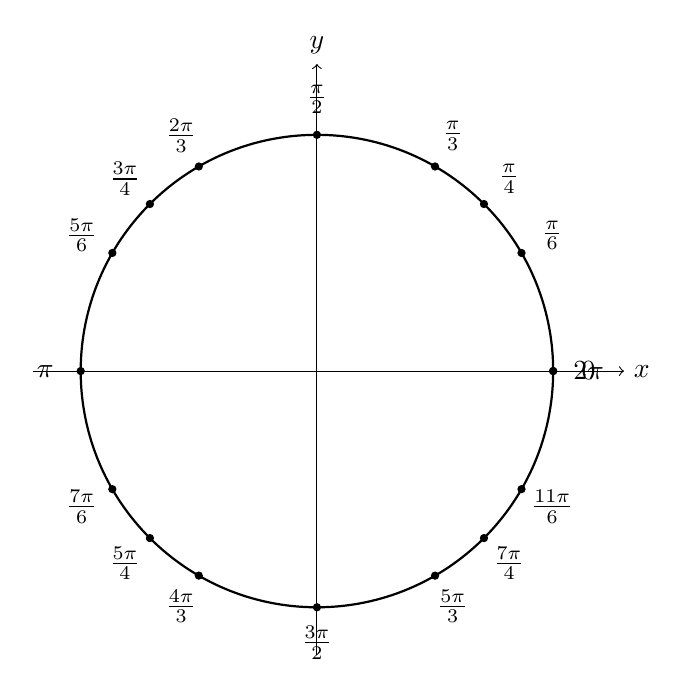
\begin{tikzpicture}[scale=3]
  % Draw the unit circle
  \draw[thick] (0,0) circle(1);

  % Axes
  \draw[->] (-1.2,0) -- (1.3,0) node[right] {\(x\)};
  \draw[->] (0,-1.2) -- (0,1.3) node[above] {\(y\)};

  % Points and angle labels
  \foreach \angle/\label in {
    0/0, 30/\frac{\pi}{6}, 45/\frac{\pi}{4}, 60/\frac{\pi}{3},
    90/\frac{\pi}{2}, 120/\frac{2\pi}{3}, 135/\frac{3\pi}{4},
    150/\frac{5\pi}{6}, 180/\pi, 210/\frac{7\pi}{6},
    225/\frac{5\pi}{4}, 240/\frac{4\pi}{3}, 270/\frac{3\pi}{2},
    300/\frac{5\pi}{3}, 315/\frac{7\pi}{4}, 330/\frac{11\pi}{6},
    360/2\pi}
  {
    \filldraw[black] ({cos(\angle)}, {sin(\angle)}) circle(0.015);
    \node at ({1.15*cos(\angle)}, {1.15*sin(\angle)}) {\(\label\)};
  }
\end{tikzpicture}
\end{center}

One radian is the angle made at the center of a circle when the arc length is equal to the radius of the circle.\\

$\theta \text{ radians} = \frac{s}{r} \Rightarrow s = r\theta$\\

$\pi = \frac{\text{circumference}}{\text{diameter}}$\\

$1^\circ = \frac{\pi}{180} \text{ radians}$\\

Trigonometric functions are special mathematical functions that originally come from studying right triangles. They relate the size of an angle in a triangle to the ratios of the lengths of the triangle's sides.\\

SOH-CAH-TOA is a mnemonic device that expresses the relationship between the basic trigonometric functions and the ratios of the sides in a right triangle.\\

The triangle definition only works for angles between 0 and $\frac{\pi}{2}$. To extend trig functions to all angles (including negative angles and angles larger then ($2\pi$ or $360^{\circ}$), mathematicians use the unit circle. Thus allowing use to use trig functions on the coordinate plane, enabling graphing and calculus.\\	

\textbf{trigonometric identities:}
\begin{itemize}
	\item $\frac{1}{\cos(\theta)} = \sec(\theta)$	
	\item $\frac{1}{\sin(\theta)} = \csc(\theta) $
	\item $\frac{1}{\tan(\theta)} = \cot(\theta)$
	\item $\sin(\theta + 2\pi) = \sin(\theta)$
	\item $\cos(\theta + 2\pi) = \cos(\theta)$
	\item $\tan(\theta + \pi) = \tan(\theta)$
	\item $\cos(\frac{\pi}{2} - \theta) = \sin(\theta)$
	\item $\sin(\frac{\pi}{2} - \theta) = \cos(\theta)$
	\item $\tan(\frac{\pi}{2} - \theta) = \cot(\theta)$
	\item $\sin(-\theta) = -\sin(\theta)$
	\item $\cos(-\theta) = \cos(\theta)$
	\item $\tan(\theta) = -\tan$
	\item $\sin^2(\theta) + \cos^2(\theta) = 1$
	\item $1 + \tan^2(\theta) = \sec^2(\theta)$
	\item $1 + \cot^2(\theta) = \csc^2(\theta)$
	\item $\cos(A \pm B) = \cos(A)\cos(B) \mp \sin(A)\sin(B)$		
	\item $\sin(A \pm B) = \sin(A)\cos(B) \pm \cos(A)\sin(B)$
	\item $\tan(A \pm B) = \frac{\tan(A) \pm \tan(B)}{1 \mp \tan(A)\tan(B)}$
	\item $\sin(2\theta) = 2\sin(\theta)\cos(\theta)$
	\item $\cos(2\theta) = \cos^2(\theta) - \sin^2(\theta)$		
	\item $\cos(2\theta) = 2\cos^2(\theta) - 1$
	\item $\cos(2\theta) = 1 - 2\sin^2(\theta)$
	\item $\cos\left(\frac{x}{2}\right) = \pm \sqrt{\frac{1 + \cos x}{2}}$
	\item $\sin\left(\frac{x}{2}\right) = \pm \sqrt{\frac{1 - \cos x}{2}}$
	\item $\tan\left(\frac{x}{2}\right) = \pm \sqrt{\frac{1 - \cos x}{1 + \cos x}}$
	\item $\tan\left(\frac{x}{2}\right) = \frac{\sin x}{1 + \cos x}$
	\item $\tan\left(\frac{x}{2}\right) = \frac{1 - \cos x}{\sin x}$
	\item $\cos A \cos B = \frac{1}{2} \left[ \cos(A - B) + \cos(A + B) \right]$
	\item $\sin A \sin B = \frac{1}{2} \left[ \cos(A - B) - \cos(A + B) \right]$
	\item $\sin A \cos B = \frac{1}{2} \left[ \sin(A + B) + \sin(A - B) \right]$
	\item $\cos A \sin B = \frac{1}{2} \left[ \sin(A + B) - \sin(A - B) \right]$
\end{itemize}

\textbf{law of sines and cosines}\\

	$\frac{\sin(A)}{a} = \frac{\sin(B)}{b} \frac{\sin(C)}{c}$\\

	$a^2 = b^2 + c^2 - 2bc\cos(A)$ (SAS or SSS)

\section*{Limits}

An indeterminate form is a mathematical expression that arises in limits where the limit cannot be directly determined from the form itself because it is ambiguous or undefined in a straightforward way.\\

\textbf{indeterminate forms:}
	\begin{itemize}
		\item $\frac{0}{0}$
		\item $\frac{\infty}{\infty}$
		\item $0 \times \infty$
		\item $\infty - \infty$
		\item $0^0$
		\item $\infty^0$
	\end{itemize}

\textbf{types of discontinuities:}
	\begin{itemize}
		\item removeable: $f(x) = \frac{(x^2 - 1)}{x - 1}$
		\item jump: the left-hand and right-hand limit at the point exist but are not equal
		\item infinite (essential): $f(x) = \frac{1}{x}$
		\item oscillatory: $f(x) = \sin(\frac{1}{x})$
	\end{itemize}

How do the values of a function behave when x approaches a number c, whether or not the function at c is defined?\\
$f(x) = \frac{\sin(x)}{x}$
$f(0) = \frac{\sin(0)}{0} = \frac{0}{0}$\\
Using a calculator you can numerically see that as $x \to 0+$ and $x \to 0-$ the function appears to approach one.\\

\textbf{limit laws} assume that $\lim_{x \to c}f(x)$ and $\lim_{x \to c}g(x)$ exist, then:
	\begin{itemize}
		\item sum law: $\lim{x \to c}(f(x) + g(x)) = \lim_{x \to c}f(x) + \lim_{x \to c}g(x)$
		\item constant multiple law: for any number k, $\lim_{x \to c}kf(x) = k\lim_{x \to c}f(x)$
		\item product law: $\lim_{x \to c}f(x)g(x) = (\lim_{x \to c}f(x))(\lim_{x \to c}g(x)$)
		\item quotient law: if $\lim_{x \to c}g(x) \neq 0$, then $\lim_{x \to c}\frac{f(x)}{g(x)} = \frac{\lim_{x \to c}f(x)}{\lim_{x \to c}g(x)}$
	\end{itemize}

\textbf{continuity at a point:} $\lim{x \to c}f(x) = f(c)$\\

\textbf{laws of continuity} assume that $f(x)$ and $g(x)$ are continuous at a point $x = c$. then the following functions area lso continuous at $x = c$:
	\begin{itemize}
		\item $f(x) + g(x)$ and $f(x) - g(x)$
		\item $kf(x)$ for any constant k
		\item $f(x)g(x)$
		\item $\frac{f(x)}{g(x)}$ if $g(c) \neq 0$
	\end{itemize}

\textbf{continuity of composite functions} let $F(x) = f(g(x))$ be a composite function. If $g$ is continuous at $x = c$ and $f$ is continuous at $x = g(c)$, then $F(x)$ is continuous at $x = c$.\\

\textbf{squeeze theorem} assume that for $x \neq c$ (in some open interval containing $c$), $l(x) \leq f(x) \leq u(x)$ and $\lim_{x \to c}l(x) = \lim_{x \to c}u(x) = L$ then $\lim_{x \to c}f(x)$ exists and $\lim_{x \to c}f(x) = L$\\

\textbf{important trigonometric limits:}
	\begin{itemize}
		\item $\lim_{\theta \to 0}\frac{\sin(\theta)}{\theta} = 1$
		\item $\lim_{\theta \to 0}\frac{1 - \cos(\theta)}{\theta} = 0$
	\end{itemize}

\textbf{intermediate value theorem:} if $f(x)$ is continuous on a closed interval $[a, b]$ and $f(a) \neq f(b)$, then for every value $M$ between $f(a)$ and $f(b)$, there exists at least one value $c \in (a, b)$ such that $f(c) = M$.\\

\textbf{existence of zeros:} if $f(x)$ is continuous on $[a, b]$ and if $f(a)$ and $f(b)$ are nonzero and have opposite signs, then $f(x)$ has a zero in $(a, b)$.\\

we can locate zeroes of functions to arbitrary accuracy using the \textbf{bisection method}.\\
$f(x) = \cos^2(x) - 2\sin(\frac{x}{4})$\\
$f(0) = 1 > 0$, $f(2) \approx -0.786 < 0$\\
we can guarantee that $f(x) = 0$ has a solution in $(0, 2)$. we can locate a zero more accurately by dividing $[0, 2]$ into two intervals $[0, 1]$ and $[1, 2]$. one of these must contain a zero of $f(x)$. to determine which, we evalutate $f(x)$ at the midpoint $m = 1$. a calculator gives $f(1) \approx -0.203 < 0$, and since $f(0) = 1$, we see that $f(x)$ takes opposite signs at the endpoints of $[0, 1]$. therefore, $(0, 1)$ must contain a zero. we discard $[1, 2]$ because both $f(1)$ and $f(2)$ are negative. the bisection method consists of continuing this process until we narrow down the location of the zero to the desired accuracty.\\

\textbf{the size of the gap:}\\
recall that the distance from $f(x)$ to $L$ is $\lvert f(x) - L\rvert$. it is convenient to refer to the quantity $\lvert f(x) - L\rvert$ as the gap between the value $f(x)$ and the limit $L$. lets reexamine the basic trigonometric limit $\lim_{x \to 0}\frac{\sin(x)}{x}$. so 1 tells us that the gap $\lvert f(x) - 1\rvert$ gets arbitrarily small when x is sufficiently close by not equal to 0. suppose we want the gap $\lvert f(x) - 1\rvert$ to be less than 0.2. how close to 0 must x be? $\lvert f(x) - 1\rvert < 0.2$ if $0 < \lvert x\rvert < 1$. if we insist instead that the gap be smaller than 0.004, we can check by zooming in $\lvert f(x) - 1\rvert < 0.004$ if $0 < \lvert x\rvert < 0.15$. it would seem that this process can be continued: by zooming in on the graph, we can find a small interval around $c = 0$ where the gap $\lvert f(x) - 1\rvert$ is smaller than any prescribed positive number. to express this in a precise fasion, we follow time-honored tradition and use the greek letters $\epsilon$ (epsilon) and $\delta$ (delta to denote small numbers specifying the size of the gap and the quantity $\lvert x - c\rvert$, respectively. in our case, $c = 0$ and $\lvert x - c\rvert = \lvert x - 0\rvert = \lvert x\rvert$. The precise meaning is that for every choice of $\epsilon > 0$, there exists some $\delta$ (depending on $\epsilon$) such that $\lvert \frac{\sin(x)}{x} - 1\rvert < \epsilon$ if $0 < \lvert x\rvert < \delta$. the number $\delta$ tells us how close is sufficiently close for a give $\epsilon$.\\

\textbf{formal definition of a limit:}\\
suppose that $f(x)$ is defined for all $x$ in an open interval containing $c$ (but not necessarily at $x = c$). then
\begin{center}$\lim_{x \to c}f(x) = L$\end{center}
if for all $\epsilon > 0$, there exists $\delta > 0$ such that
\begin{center}$\lvert f(x) - L\rvert < \epsilon$ if $0 < \lvert x - c\rvert < \delta$\end{center}

four rigorous definitions of the limit:
	\begin{itemize}
		\item $\lim_{x \to a}f(x) = L$ means $\forall \epsilon > 0, \exists \delta > 0 : 0 < \lvert x - a\rvert < \delta \Rightarrow \lvert f(x) - L\rvert < \epsilon$
		\item $\lim_{x \to \infty}f(x) = L$ means $\forall \epsilon > 0, \exists N > 0 : x > N \Rightarrow \lvert f(x) - L\rvert < \epsilon$   
		\item $\lim_{x \to a}f(x) = \infty$ means $\forall M > 0, \exists \delta > 0 : 0 < \lvert x - a\rvert < \delta \Rightarrow f(x) > M$  
		\item $\lim_{x \to \infty}f(x) = \infty$ means $\forall M > 0, \exists N > 0 : x > N \Rightarrow f(x) > M$
	\end{itemize}

\section*{Differentiation}

\textbf{the derivative} of a function $f$ at $x = a$ is the limit of the difference quotients (if it exists):
\begin{center} $f'(a) = \lim_{h \to 0}\frac{f(a + h) - f(a)}{h}$ \end{center}
when the limit exists, we say that $f$ is differentiable at $x = a$. an equivalent definition of the derivative is
\begin{center} $f'(a) = \lim_{x \to a}\frac{f(x) - f(a)}{x - a}$ \end{center}

\textbf{tangent lines:}\\
assume that $f(x)$ is differentiable at $x = a$. the tangent line to the graph of $y = f(x)$ at $P = (a, f(a))$ is the line through $P$ of slope $f'(a)$. the equation of the tangent line in point-slope form is
\begin{center} $y - f(a) = f'(a)(x - a)$ \end{center}

\textbf{derivative of linear and constant functions:}
	\begin{itemize}
		\item if $f(x) = mx + b$ is a linear function, then $f'(a) = m$ for all $a$
		\item if $f(x) = b$ is a constant function, then $f'(a) = 0$ for all $a$
	\end{itemize}

\textcolor{blue}{proof of the power rule}
	\begin{enumerate}
		\item assume that $n$ is a whole number and let $f(x) = x^n$. then $f'(a) = \lim_{x \to a}\frac{x^n - a^n}{x - a}$
		\item to simplify the difference quotient, we need to generalize the following identities: $x^2 - a^2 = (x - a)(x + a)$\\ $x^3 - a^3 = (x - a)(x^2 + xa + a^2)$\\ $x^4 - a^4 = (x - a)(x^3 + x^2a + xa^2 + a^3)$
		\item the generalizaiton is $x^n - a^n = (x - a)(x^{n - 1} + x^{n - 2}a + x^{n - 3}a^2 + \ldots + xa^{n - 2} + a^{n - 1})$
		\item to verify, observe that the right-hand side is equal to\\ $x(x^{n - 1} + x^{n - 2}a + x^{n - 3}a^2 + \ldots + xa^{n - 2} + a^{n - 1})$\\$-a(x^{n - 1} + x^{n - 2}a + x^{n - 3}a^2 + \ldots + xa^{n - 2} + a^{n - 1})$
		\item when we carry out the multiplications, al terms cancle except the first and the last, so $x^n - a^n$ remains, as required. the identity gives us\\ $\frac{x^n - a^n}{x - a} = x^{n - 1} + x^{n - 2}a + x^{n - 3}a^2 + \ldots + xa^{n - 2} + a^{n - 1} (x \neq a)$
		\item therefore,\\ $f'(a) = \lim_{x \to a}(x^{n - 1} + x^{n - 2}a + x^{n - 3}a^2 + \ldots + xa^{n - 2} + a^{n - 1})$\\ $a^{n - 1} + a^{n - 2}a + a^{n - 3}a^2 + \ldots + aa^{n - 2} + a^{n - 1} (\text{n terms})$\\ $na^{n - 1}$
	\end{enumerate}

\textbf{linearity rules} assume that $f$ and $g$ are differentiable functions
	\begin{itemize}
		\item sum rule: the function $f + g$ is differentiable and $(f + h)' = f' + g'$
		\item constant multiple rule: for any constant $c$, $cf$ is differentiable and $(cf)' = cf'$
	\end{itemize}

\textbf{differentiability implies continuity} if $f$ is differentiable at $x = c$, then $f$ is continuous at $x = c$.\\
\textcolor{blue}{Proof:}
	\begin{enumerate}
		\item by definition, if $f$ is differentiable at $x = c$, then the following limit exists: $f'(c) = \lim_{x \to c}\frac{f(x) - f(c)}{x - c}$
		\item our goal is to prove that $f$ is continuous at $x = c$, which means that $\lim_{x \to c}f(x) = f(c)$. To relate the two limits, consider the equation (valid for $x \neq c$) $f(x) - f(c) = (x - c)\frac{f(x) - f(c)}{x - c}$
		\item both factors on the right approach a limit as $x \to c$, so we may apply the limit laws: $\lim_{x \to c}(f(x) - f(c)) = \lim_{x \to c}((x - c)\frac{f(x) - f(c)}{x - c})$
		\item $\lim_{x \to c}(f(x) - f(c)) = (\lim_{x \to c}(x - c)(\lim_{x \to c}\frac{f(x) - f(c)}{x - c})$
		\item $\lim_{x \to c}(f(x) - f(c)) = 0 \cdot f'(c) = 0$
		\item therefore, $\lim_{x \to c}f(x) = \lim_{x \to c}(f(x) - f(c)) + \lim_{x \to c}f(c) = 0 + f(c) = f(c)$, as desired
	\end{enumerate}

\textcolor{blue}{proof of the product rule}
	\begin{enumerate}
		\item we prove the product rule by writing the difference quotient for $f(x)g(x)$ in a vlever way as a sum of two terms. the limit definition of the derivative applied to the product function gives us\\ $(fg)'(x) = \lim_{h \to 0}\frac{f(x + h)g(x + h) - f(x)g(x)}{h}$
		\item the trick is to subtract $f(x + h)g(x)$ and add it back again in the numerator of the difference quotient:\\ $f(x + h)g(x + h) - f(x + h)g(x) + f(x + h)g(x) - f(x)g(x)$
		\item combing terms, we see that the numerator is equal to\\ $f(x + h)(g(x + h) - g(x)) + g(x)(f(x + h) - f(x))$
		\item now write $(fg)'(x)$ as a sum of two limits: \\ $(fg)'(x) = \lim_{h \to 0}f(x + h)\frac{g(x + h) - g(x)}{h} + \lim_{h \to 0}g(x)\frac{f(x + h) - f(x)}{h}$
		\item the use of the sum law is valid, provided that each limit on the right exists. to check that the first limit exist and evaluate it, we note that $f(x)$ is continuous (because it is differentiable) and that $g(x)$ is differentiable:\\ $\lim_{h \to 0}f(x + h)\frac{g(x + h) - g(x)}{h} = \lim_{h \to 0}f(x + h)\lim_{h \to 0}\frac{g(x + h) - g(x)}{h} = f(x)g'(x)$
		\item the second limit is similar:\\ $\lim_{h \to 0}g(x)\frac{f(x + h) - f(x)}{h} = g(x)\lim_{h \to 0}\frac{f(x + h) - f(x)}{g} = g(x)f'(x)$
		\item using the aforementioned we conclude that $fg$ is differentiable and that $(fg)'(x) = f(x)g'(x) + g(x)f'(x)$ as desired.
	\end{enumerate}		

\textcolor{blue}{proof of the quotient rule}
	\begin{enumerate}
		\item start with the definition of the derivative\\ $(\frac{f}{g})'(x) = \lim_{h \to 0}\frac{\frac{f(x + h)}{g(x + h)} - \frac{f(x)}{g(x)}}{h}$
		\item combine the two fractions in the numerator\\ $(\frac{f}{g})'(x) = \lim_{h \to 0} \frac{1}{h} \cdot \frac{f(x + h)g(x) - f(x)g(x + h)}{g(x + h)g(x)}$    
		\item manipulate the numerator\\ $f(x + h)g(x) - f(x)g(x + h) = [f(x + h)g(x) - f(x)g(x)] - [f(x)g(x + h) - f(x)g(x)] = g(x)[f(x + h) - f(x)] - f(x)[g(x + h) - g(x)]$
		\item lets put that back into the limit\\ $(\frac{f}{g})'(x) = \lim_{h \to 0}\frac{g(x)[f(x + h) - f(x)] - f(x)[g(x + h) - g(x)]}{h \cdot g(x + h)g(x)}$ 
		\item split the limit\\ $\lim_{h \to 0}[\frac{g(x)[f(x + h) - f(x)]}{h \cdot g(x + h)g(x)} - \frac{f(x)[g(x + h) - g(x)]}{h \cdot g(x + h)g(x)}]$\\
		\item $(\frac{f}{g})'(x) = \frac{g(x)f'(x) - f(x)g'(x)}{[g(x)]^2}$ 
	\end{enumerate}

\textcolor{blue}{proof of the derivative of sin}
	\begin{enumerate}
		\item $\sin(x + h) = \sin(x)\cos(h) + \cos(x)\sin(h)$
		\item $\sin(x + h) - \sin(x) = \sin(x)\cos(h) + \cos(x)\sin(h) - \sin(x)$ 
		\item $\sin(x + h) - \sin(x) = (\sin(x)\cos(h) - \sin(x)) + \cos(x)\sin(h)$ 
		\item $\sin(x + h) - \sin(x) = \sin(x)(\cos(h) - 1) + \cos(x)\sin(h)$ 
		\item $\lim_{h \to 0}\frac{\sin(x)(\cos(h) - 1)}{h} + \lim_{h \to 0}\frac{\cos(x)\sin(h)}{h}$
		\item $\sin(x)(0) + \cos(x)(1)$
	\end{enumerate}

\textcolor{blue}{proof of the chain rule}
	\begin{enumerate}
		\item $h(x) = f(g(x))$
		\item $h'(x) = \lim_{h \to 0}\frac{f(g(x + h)) - f(g(x))}{h}$
		\item the key idea is to manipulate the difference quotient to introduce $g(x + h) - g(x)$\\ $\frac{f(g(x + h)) = f(g(x))}{h} = \frac{f(g(x + h)) - f(g(x))}{g(x + h) - g(x)} \cdot \frac{g(x + h) - g(x)}{h}$
		\item $h'(x) = \lim_{h \to 0}\frac{f(g(x + h)) - f(g(x))}{g(x + h) - g(x)} \cdot \lim_{h \to 0}\frac{g(x + h) - g(x)}{h}$
		\item this is legitimate only if the denominator $g(x + h - g(x)$ is nonzero. therefore, to continue our proof, we make the extra assumption that $g(x + h) - g(x) \neq 0$ for all $h$ near but not equal to 0. this assumption is not necessary, but without it, the argument is more technical. the second limit on the right is $g'(x)$. the chain rule will follow if we show that the first limit equals $f'(g(x))$. to verify this, set $k = g(x + h) - g(x)$. then $g(x + h) = g(x) + k$ and\\ $\frac{f(g(x + h) - f(g(x)}{g(x + h) - g(x)} = \frac{f(g(x) + k) - f(g(x)}{k}$
		\item since $g(x)$ is differentiable, it is also continuous. therefor $g(x + h)$ tends to $g(x)$ and $k = g(x + h) - g(x)$ tends to zero as $h \to 0$. thus, we may rewrite the limit in terms of $k$ to obtain the desired result:\\ $\lim_{h \to 0}\frac{f(g(x + h)) - f(g(x))}{g(x + h) - g(x)} = \lim_{k \to 0}\frac{f(g(x) + k - f(g(x))}{k} = f'(g(x))$
	\end{enumerate}

\textcolor{blue}{proof of the general power rule}
	\begin{enumerate}
		\item we write $g(x)^n = f(g(x))$, with $f(u) = u^n$. then $f'(u) = nu^{n - 1}$ and, by the chain rule,\\ $\frac{d}{dx}(g(x))^n = f'(g(x))g'(x) = n(g(x))^{n - 1}g'(x)$
	\end{enumerate}

\textbf{shifting and scaling rule} if $f(x)$ is differentiable, then for any constants $k$ and $b$, $\frac{d}{dx}f(kx + b) = kf'(kx + b)$\\

\textbf{implicit differentiation:}\\
to differentiate using the methods covered thus far, we must have a formula for $y$ in terms of $x$, for instance, $y = x^3 + 1$. but suppose that $y$ is determined instead by an equation such as $y^4 + xy = x^3 - x + 2$. in this case, we say that $y$ is defined impplicitly. how can we find the slope of the tangent line at a point on the graph? it may be inconvenient or even impossible to solve for $y$ explicitly as a function of $x$, but we can find $\frac{dy}{dx}$ using the method of implicit differentiation. to illustrate, consider the equation of the unit circle:
	\begin{enumerate}
		\item $x^2 + y^2 = 1$
		\item to compute $\frac{dy}{dx}$, first take the derivative of both sides of the equation and evaluate: \\ $\frac{d}{dx}(x^2 + y^2) = \frac{d}{dx}(1)$
		\item $\frac{d}{dx}(x^2) + \frac{d}{dx}(y^2) = 0$
		\item $2x + \frac{d}{dx}(y^2) = 0$
		\item what should we do with the term $\frac{d}{dx}(y^2)$? we use the chain rule. if we think of $y$ as a function $y = f(x)$, then $y^2 = f(x)^2$, and by the chain rule,\\ $\frac{d}{dx}y^2 = \frac{d}{dx}f(x)^2 = 2f(x)\frac{df}{dx} = 2y\frac{dy}{dx}$
		\item $2x + \frac{d}{dx}(y^2)\to 2x + 2y\frac{dy}{dx}$, and we may solve for $\frac{dy}{dx}$ if $y \neq 0$:
		\item $\frac{dy}{dx} = -\frac{x}{y}$
	\end{enumerate}

\textbf{related rates:}\\
in related rate problems, the goal is to calculate an unknown rate of change in terms of other rates of change that are known. one typical problem involves a ladder learning against a wall. the question is: how fast does the ladder move if the bottom of the ladder is pulled away from the wall at constant speed? what is interesting and perhaps surprising is that the top and bottom travel at different speeds.\\

\textbf{linear approximation:}\\
we can use the derivative to estimate $\Delta f$ without computing it exactly. by definition, the derivative is the limit\\ $f'(a) = \lim_{\Delta x \to 0}\frac{f(a + \Delta x) - f(a)}{\Delta x} = \lim_{\Delta x \to 0}\frac{\Delta f}{\Delta x}$\\ so when $\Delta x$ is small, we have $\frac{\Delta f}{\Delta x} \approx f'(a)$, and thus, $\Delta f \approx f'(a)\Delta x$\\

the linear approximation if often called the tangent line approximation because of the following interpretation. the quantitiy $\Delta f$ is the vertical change from $x = a$ to $a = a + \Delta x$ in the graph of $f(x)$. recall that for a nonvertical straight line, the vertical change is equal to the slope times the horizontal change. since the tangent line has slope $f'(a)$. the vertical change in the tangent line is $f'(a)\Delta x$. what the linear approximation does, therefore, is used the vertical change in the tangent line as an approximation to the vertical change in the graph of $f(x)$. when $\Delta x$ is small, the two quantities are nearly equal.\\

Keep in mind the different roles played by $\Delta f$ and $f'(a)\Delta x$. the quantity of interest is $\Delta f$ and we estimate it by $f'(a)\Delta x$. most importantly, the linear approximation tells us that there is a nearly linear relationship between $\Delta f$ and $\Delta x$ when $\Delta x$ is small.\\

\textbf{linearization:}\\
we can approximate $f(x)$ itself rather than the change $\Delta f$ by rewriting the linear approximation in terms of the variable $x = a + \Delta x$. Then\\ $f(a + \Delta x) - f(a) \approx f'(a)\Delta x$\\ $f(x) - f(a) \approx f'(a)(x - a)$ (since $\Delta x = x - a$)\\ $f(x) \approx f(a) + f'(a)(x - a)$\\ the function on the right, denoted by $L(x)$, is called the linearization of $f(x)$ at $x = a$:\\ $L(x) = f'(a)(x - a) + f(a)$\\ we refer to $x = a$ as the center of the linearization. notice that $y = L(x)$ is the equation of the tangent line to the graph of $f(x)$ at $x = a$\\

\textbf{approximating $f(x)$ by its linearization} assume that $f$ is differentiable at $x = a$ if $x$ is close to $a$, then\\ $f(x) \approx L(x) = f'(a)(x - a) + f(a)$\\

\textbf{extreme values on an interval} let $f(x)$ be a function on an interval I and let $a \in I$. we say that $f(a)$ is the
	\begin{itemize}
		\item absolute minimum of $f(x)$ on $I$ if $f(a) \leq f(x)$ for all $x \in I$
		\item absolute maximum of $f(x)$ on $I$ if $f(a) \geq f(x)$ for all $x \in I$
	\end{itemize}

\textbf{existence of extrema on a closed interval} if $f(x)$ is a continuous function on a closed (bounded) interval $I = [a, b]$, then $f(x)$ takes on a minimum and a maximum value on $I$.\\

\textbf{local extrema} we say that $f(x)$ has a
	\begin{itemize}
		\item at $x = c$ if $f(c)$ is the minimum value of $f$ on some open interval (in the domain of $f$) containing $c$.
		\item at $x = c$ if $f(c)$ is the maximum value of $f(x)$ on some open interval (in the domain of $f$) containing $c$.
	\end{itemize}

\textbf{critical points} a number $c$ in the domain of $f$ is called a critical point if either $f'(c) = 0$ or $f'(c)$ DNE.\\

\textbf{fermat's theorem on local extrema} if $f(c)$ is a local min or max, then $c$ is a critical point of $f$.\\

\textbf{extreme values on a closed interval} assume that $f(x)$ is continuous on $[a, b]$ and let $f(c)$ be the minimum or maximum value on $[a, b]$. then $c$ is either a critical point or one of the endpoints $a$ or $b$.\\

\textbf{rolle's theorem} assume that $f(x)$ is continous on $[a, b]$ and differentiable on $(a, b)$. if $f(a) = f(b)$, then there exists a number $c$ between $a$ and $b$ such that $f'(c) = 0$.\\

\textbf{mean value theorem} assume that $f$ is continuous on the closed interval $[a, b]$ and differentiable on $(a, b)$. then there exists at least one value $c$ in $(a, b)$ such that\\ $f'(c) = \frac{f(b) - f(a)}{b - a}$\\

\textbf{the sign of the derivative} let $f$ be a differentiable function on the open interval $(a, b)$.
	\begin{itemize}
		\item if $f'(x) > 0$ for $x \in (a, b)$, then $f$ is increasing on $(a, b)$.
		\item if $f'(x) < 0$ for $x \in (a, b)$, then $f$ is decreasing on $(a, b)$. 
	\end{itemize}

\textbf{first derivative test for critical points} assume that $f(x)$ is differentiable and let $c$ be a critical point of $f(x)$. then:
	\begin{itemize}
		\item $f'(x)$ changes from + to - at $c$ $\Rightarrow$ $f(c)$ is a local maximum.
		\item $f'(x)$ changes from - to + at $c$ $\Rightarrow$ $f(c)$ is a local minimum. 
	\end{itemize}

\textbf{test for concavity} suppose that $f''(x)$ exists for all $x \in (a, b)$.
	\begin{itemize}
		\item if $f''(x) > 0$ for all $x \in (a, b)$, then $f$ is concave up on $(a, b)$.
		\item if $f''(x) < 0$ for all $x \in (a, b)$, then $f$ is concave down on $(a, b)$. 
	\end{itemize}

\textbf{test for inflection points} assume that $f''(x)$ exists for all $x \in (a, b)$ and let $c \in (a, b)$. if $f''(c) = 0$ and $f''(x)$ changes sign at $x = c$, then $f(x)$ has a point of inflection at $x = c$.\\

\textbf{second derivative test} assume that $f(x)$ is differentiable and let $c$ be a critical point. if $f''(c)$ exists, then
	\begin{itemize}
		\item $f''(c) > 0 \Rightarrow f(c)$ is a local minimum
		\item $f''(c) < 0 \Rightarrow f(c)$ is a local maximum 
		\item $f''(c) = 0 \Rightarrow f(c)$ inconclusive: $f(c)$ may be a local min, max, or neither
	\end{itemize}

\textbf{newton's method:}\\
this is a procedure for finding numerical approximations to zeros of functions. numerical approximations are important because it is often impossible to find the zeros exactly. for example, the polynomial $f(x) = x^5 - x - 1$ has one real root $c$, but we can prove, using an advanced branch of mathematics called Galois Theory, that there is no algebraic formula for this root. newtons method shows that $c \approx 1.1673$, and with enough computation, we can compute $c$ to any desired degree of accuracy.\\

in newton's method, we begin by choosing a number $x_0$, which we believe is close to a root of $f(x)$. this starting value $x_0$ is called the initial guess. newton's method then produces a sequence $x_0, x_1, x_2, \ldots$ of successive approximations that, in favorable situations, converge to a root.\\

steps:
	\begin{itemize}
		\item choose initial guess $x_0$ (close to the desired root if possible).
		\item generate successive approximations $x_1, x_2, \ldots$ where\\ $x_{n + 1} = x_n - \frac{f(x_n)}{f'(x_n)}$
	\end{itemize}

\textbf{derivatives:}
	\begin{itemize}
		\item $\frac{d}{dx}(c) = 0$
		\item $\frac{d}{dx}x = 1$
		\item $\frac{d}{dx}(x^n) = nx^{-1}$ (power rule)
		\item $\frac{d}{dx}[cf(x)] = cf'(x)$
		\item $\frac{d}{dx}[f(x)+g(x)] = f'(x) + g'(x)$
		\item $\frac{d}{dx}[f(x)g(x)] = f(x)g'(x) + g(x)f'(x)$
		\item $\frac{d}{dx}[\frac{f(x)}{g(x)}] = \frac{g(x)f'(x) - f(x)g'(x)}{[g(x)]^2}$
		\item $\frac{d}{dx}f(g(x)) = f'(g(x))g'(x)$
		\item $\frac{d}{dx}f(x)^n = nf(x)^{n-1}f'(x)$
		\item $\frac{d}{dx}\sin(x) = \cos(x)$
		\item $\frac{d}{dx}\cos(x) = -\sin(x)$
		\item $\frac{d}{dx}\tan(x) = \sec^2(x)$
		\item $\frac{d}{dx}\csc(x) = -\csc(x)\cot(x)$
		\item $\frac{d}{dx}\sec(x) = \sec(x)\tan(x)$
		\item $\frac{d}{dx}\cot(x) = -\csc^2(x)$
		\item $\frac{d}{dx}\sin^{-1}(x) = \frac{1}{\sqrt(1 - x^2)}$
		\item $\frac{d}{dx}\cos^{-1}(x) = -\frac{1}{\sqrt(1 - x^2)}$
		\item $\frac{d}{dx}\tan^{-1}(x) = \frac{1}{1 + x^2}$
		\item $\frac{d}{dx}(e^x) = e^x$
		\item $\frac{d}{dx}(a^x) = (\ln a)a^x$
		\item $\frac{d}{dx}\ln\mid x\mid = \frac{1}{x}$
		\item $\frac{d}{dx}\log_ax = \frac{1}{(\ln a)x}$
	\end{itemize}

\section*{Integration}
\textbf{antiderivatives} a function $F(x)$ is an antiderivative of $f(x)$ on $(a, b)$ if $F'(x) = f(x)$ for all $x \in (a, b)$.\\

\textbf{general antiderivative} let $F(x)$ be an antiderivative of $f(x)$ on $(a, b)$. then every other antiderivative on $(a, b)$ is of the form $F(x) + C$ for some constant $C$.\\

\textbf{indefinite integral} the notion $\int f(x)\,dx = F(x) + C$ means that $F'(x) = f(x)$ we say that $F(x) + C$ is the antiderivative or indefinite integral of $f(x)$.\\

\textbf{power rule for integrals} $\int x^n\,dx = \frac{x^{n + 1}}{n + 1} + C$ for $n \neq -1$\\ 

\textbf{linearity of the indefinite integral:}
	\begin{itemize}
		\item $\int (f(x) + g(x))\,dx = \int f(x)\,dx + \int g(x)\,dx$
		\item $\int cf(x)\,dx = c\int f(x)\,dx$
	\end{itemize}

\textbf{basic trigonometric integrals:}
	\begin{itemize}		
		\item $\int \sin x \,dx = -\cos x + C$
		\item $\int \cos x \,dx = \sin x + C$
		\item $\int \sec^2 x \,dx = \tan x + C$
		\item $\int \csc^2 x \,dx = -\cot x + C$
		\item $\int \sec x \tan x \,dx = \sec x + C$
		\item $\int \csc x \cot x \,dx = -\csc x + C$
	\end{itemize}

for the rest of this section assume that $f(x)$ is continuous and positive, so that the graph of $f(x)$ lies above the x-axis. as a first step, we approximate the area using rectangles. first, choose a whole number $N$ and divide $[a, b]$ into $N$ subintervals of equal width, each subinterval has width $\Delta x = \frac{b - a}{N}$ since $[a, b]$ has width $b - a$. the right endpoints of the subintervals are $a + \Delta x, a + 2\Delta x, \ldots, a + (N - 1)\Delta x, a + N\Delta x$. notice that the last right enpoint is $b$ because $a + N\Delta x = a + N(\frac{b - a}{N}) = b$. next, above each subinterval, construct the rectangle whose height is the value of $f(x)$ at the right enpoint of the subinterval. each rectangle has width $\Delta x$. the height of the first rectangle is $f(a + \Delta x)$ and its area is $f(a + \Delta x)\Delta x$. similarly, the second rectangle ahs a height $f(a + 2\Delta x)$ and area of $f(a + 2\Delta x)\Delta x$, ect. the sum of the areas of the rectangles is $f(a + \Delta x)\Delta x + f(a + 2\Delta x)\Delta x + \ldots + f(a + N\Delta x)\Delta x$. this sum is called the Nth right-endpoint approximation and is denoted $R_N$ as $R_N = \Delta x[f(a + \Delta x) + f(a + 2\Delta x) + \ldots + f(a + N\Delta x)]$. in words, $R_N$ is equal to $\Delta x$ times the sum of the function values at the right endpoints of the subintervals.\\

\textbf{linearity of summations}
	\begin{itemize}
		\item $\sum_{j=m}^{n}(a_j + b_j) = \sum_{j=m}^{n}a_j + \sum_{j=m}^{n}b_j$
		\item $\sum_{j=m}^{n}Ca_j = C\sum_{j=m}^{n}a_j$ ($C$ any constant)
		\item $\sum_{j=1}^{n}k = nk$ ($k$ for any constant and $n \geq 1$)
	\end{itemize}

$R_N = \Delta x[f(a + \Delta x) + f(a + 2\Delta x) + \ldots + f(a + N\Delta x)]$\\
$R_N = \Delta x\sum_{j=1}^{N}f(a + j\Delta x)$\\
$L_N = \Delta x[f(a) + f(a + \Delta x) + f(a + 2\Delta x) + \ldots + f(a + (N -1)\Delta x)]$\\
$L_N = \Delta x\sum_{j=0}^{N-1}f(a + j\Delta x)$\\
$M_N = \Delta x\sum_{j=1}^{N}f(a + (j - \frac{1}{2})\Delta x)$\\

if $f(x)$ is continuous on $[a, b]$, then the endpoint and midpoint approximations approach one and the same limit as as $N \to \infty$. in other words, there is a value $L$ such that $\lim_{N \to \infty}R_N = \lim_{N \to \infty}L_N = \lim_{N \to \infty}M_N = L$\\

\textbf{power sums}\\
the kth power sum is the sum of the kth powers of the first $N$ integers.\\
	\begin{itemize}
		\item $\sum_{j=1}^{N}j = 1 + 2 + \ldots + N = \frac{N(N + 1)}{2} = \frac{N^2}{2} + \frac{N}{2}$
		\item $\sum_{j=1}^{N}j^2 = 1^2 + 2^2 + \ldots + N^2 = \frac{N(N + 1)(2N + 1)}{6} = \frac{N^3}{3} + \frac{N^2}{2} + \frac{N}{6}$ 
		\item $\sum_{j=1}^{N}j^3 = 1^3 + 2^3 + \ldots + N^3 = \frac{N^2(N + 1)^2}{4} = \frac{N^4}{4} + \frac{N^3}{2} + \frac{N^2}{4}$ 
	\end{itemize}

in the endpoint and midpoint approximations, we approximate the area under the graph by rectangles of equal width. the heights of the rectangles are the values of $f(x)$ at the endpoints or midpoints of the subintervals. in riemann sum approximations, we relax these requirements; the rectangles need not have equal width and height of a rectangle may be any value of $f(x)$ within the subinterval. more formally, to define a riemann sum, we choose a partition and a set of intermediate points. a partition $P$ of length $N$ is any choice of points in $[a, b]$ that divides the interval into $N$ subintervals:\\
partition P: $a = x_0 < x_1 < x_2 \ldots < x_N = b$\\
subintervals: $[x_0, x_1], [x_1, x_2], \ldots [x_{N-1}, x_{N}]$\\
we denote the length of the ith interval by $\Delta x_i = x_i - x_i - x_{i-1}$\\
the maximum of the lendths $\Delta x_i$ is called the norm of the partition $P$ and is denoted $\lVert P\rVert$. a set of intermediate points is a set of points $C = {c_1, \ldots, c_N}$, where $c_i$ belongs to $[x_{i-1}, x_i]$\\

now, over each subinterval $[x_{i-1}, x_i]$ we constuct the rectangle of height $f(c_i)$ and base $\Delta x_i$. this rectangle has area $f(c_i)\Delta x_i$. if $f(c_i) < 0$, the rectangle extends below the x-axis and the "area" $f(c_i)\Delta x_i$ is negative. the riemann sum is the sum of these positive or negative areas: $R(f, P, C) = \sum_{i=1}^{N}f(c_i)\Delta x_i = f(c_1)\Delta x_1 + f(c_2)\Delta x_2 + \ldots + f(c_N)\Delta x_N$\\

the endpoint and midpoint approximations are examples of riemann sums. they correspond to the partition of $[a, b]$ into $N$ subintervals of equal length $\Delta x = \frac{b - a}{N}$ and the choice of right endpoints, left endpoints, or midpoints as intermediate points.\\

having introduced riemann sums, we are ready to make the following definition: a function is integrable of $[a, b]$ if all of the riemann sum (not just the endpoint and midpoint approximations) approach one and the same limit $L$ as the norm of the partition tends to zero. more formally, we write\\
$L = \lim_{\lVert P\rVert \to 0}R(f, P, C) = \lim_{\lVert P\rVert \to 0}\sum_{i=1}^{N}f(c_i)\Delta x_i$\\
if $\lvert R(f, P, C) - L\rvert$ gets arbitrarily small as the norm $\lVert P\rVert$ tends to zero, no matter how we choose the partition and intermediate points. note that as $\lVert P\rVert \to 0$, the number $N$ of intervals tends to $\infty$. the limit $L$ is called the definite integral of $f(x)$ over $[a, b]$.\\

\textbf{definite integral}\\
the definite integral of $f(x)$ over $[a, b]$ is the limit of riemann sums and is denoted by the integral sign:\\
$\int_{a}^{b}f(x)\, dx = \lim_{\lVert P\rVert \to 0}R(f, P, C) = \lim_{\lVert P\rVert \to 0}\sum_{i=1}^{N}f(c_i)\Delta x_i$\\
when this limit exists, we say that $f(x)$ is integrable over $[a, b]$.\\

\textcolor{blue}{remarks}
	\begin{itemize}
		\item we often refer to the definite integral more simply as the integral of $f$ over $[a, b]$.
		\item the function $f(x)$ inside the integral sign is called integrand
		\item the numbers $a$ and $b$ representing the interval $[a, b]$ are called the limits of integration.
		\item any variable may be used as a variable of integration (this is a "dummy" variable). thus, the following three integrals all denote the same quantitiy: $\int_{a}^{b}f(x)\,dx$, $\int_{a}^{b}f(t)\,dt$, $\int_{a}^{b}f(u)\,du$  
		\item recall that the indefinite integral $\int f(x)\, dx$ denotes the general antiderivative of $f(x)$
	\end{itemize}
most functions that arise in practice are integrable. in particular, every continuous function is integrable, as stated in the following theorem.\\
if $f(x)$ is continuous on $[a, b]$, then $f(x)$ is integrable over $[a, b]$.\\

when $f(x)$ is continuous and positive, we interpret the definite integral as the area under the graph. if $f(x)$ is not positive, then the definite integral is not equal to an area in the usual sense, but we may interpret is as the signed area between the graph and the x-axis. signed area is defined as following:\\
signed area of a region $=$ (area above x-axis) - (area below x-axis)\\

thus, signed area treats regions under the x-axis as "negative area". to see why the definit eintegral gives us signed area, suppose first that $f(x)$ is negative on $[a, b]$ and consider a riemann sum: $R(f, C, P) = f(c_1)\Delta x_1 + f(c_2)\Delta x_2 + \ldots + f(c_N)\Delta x_N$ since $f(c_i) < 0$, each term is equal to the negative of the area of a rectangle: $f(c_i)\Delta x_i = -(\text{area of rectangle of height }\lvert f(c_i)\rvert)$\\

therefore, the riemann sums $R(f, C, P)$ converge to the negative of the area between the graph and the x-axis. if $f(x)$ takes on both positive and negative values, then $f(c_i)\Delta x_i$ is positive or negative, depending on whether the corresponding rectangle lies above or below the x-axis. in this case, the riemann sums converge to the signed area. in summary,\\
$\int_{a}^{b}f(x)\, dx = \text{signed area of region between the graph and x-axis over } [a, b]$\\

\textbf{integral of a constant} for any constant $C$, $\int_{a}^{b}C\,dx = C(b - a)$.\\

\textbf{linearity of the definite integral} if $f(x)$ and $g(x)$ are integrable over $[a, b]$, then
	\begin{itemize}
		\item $\int_{a}^{b}(f(x) + g(x))\,dx = \int_{a}^{b}f(x)\,dx + \int_{a}^{b}g(x)\,dx$
		\item $\int_{a}^{b}Cf(x)\,dx = C\int_{a}^{b}f(x)\,dx$ for any constant $C$
	\end{itemize}

\textbf{reversing the limits of integration} for $a < b$, we set $\int_{a}^{b}f(x)\,dx = -\int_{b}^{a}f(x)\,dx$\\

\textbf{additivity for adjacent intervals} for $a \leq b \leq c$,\\
$ \int_{a}^{c}f(x)\,dx  = \int_{a}^{b}f(x)\,dx + \int_{b}^{c}f(x)\,dx$\\

\textbf{comparison theorem} if $g(x) \leq f(x)$ on an interval $[a, b]$, then\\
$\int_{a}^{b}g(x)\,dx \leq \int_{a}^{b}f(x)\,dx$\\

\textbf{the fundamental theorem of calculus, part I} assume that $f(x)$ is continuous on $[a, b]$ and let $F(x)$ be an antiderivative of $f(x)$ on $[a, b]$. then\\
$\int_{a}^{b}f(x)\,dx = F(b) - F(a)$\\

part I of the fundamental theorem shows that we can compute definite integrals using antiderivatives. part II turns this relationship around: it tells us that we can use the definite integral to construct antiderivatives. to state part II, we introduce the area function (or cumulative area function) associated to a function $f(x)$ and lower limit $a$: $A(x) = \int_{a}^{x}f(t)\, dx = \text{signed area from a to x}$ in essence, we turn the definite integral into a function by trating the upper limit x as a variable rather than a constant. notice that $A(a) = 0$ because $A(a) = \int_{a}^{a}f(t)\,dt = 0$. although $A(x)$ is defined by an integral, in many cases we can find an explicit formula it.\\

\textbf{fundamental theorem of calculus, part II} let $f(x)$ be a continuous function on $[a, b]$. then $A(x) = \int_{a}^{x}f(t)\, dt$ is an antiderivative of $f(x)$, that is, $A'(x) = f(x)$, or equivalently,\\
$\frac{d}{dx}\int_{a}^{x}f(t)\,dt = f(x)$\\
furthermore, $A(x)$ satisfies the initial condition $A(a) = 0$.\\

integration (antidifferentiation) is generally more difficult than differentiation. there are no sure-fire methods for finding an antiderivative, and, in some cases, there is no elementary formula for the antiderivative. however, there are several general techniques that are widely applicable. one such technique is the substitution method, which uses the chain rule "in reverse".\\

\textbf{substitution method} if $F'(x) = f(x)$, then\\
$\int f(u(x))u'(x)\,dx = F(u(x)) + C$\\

there are two ways of using substitution to compute definite integrals. one way is to carry out the substitution method fully to find an antiderivative in terms of the x-variable. however, it is often more efficient to evaluate the definite integral directly in terms of the u-variable. this can be done provided that the limits of integration are changed as indicated in the next theorem.\\

\textbf{change of variables formula for definite integrals} if $u(x)$ is differentiable on $[a, b]$ and $f(x)$ is integrable on the range of $u(x)$, then\\
$\int_{a}^{b}f(u(x))u'(x)\,dx = \int_{u(a)}^{u(b)}f(u)\,du$\\

$\text{area between the graphs} = \int_{a}^{b}(y_{\text{top}} - y_{\text{bot}})\,dx = \int_{a}^{b}(f(x) - g(x))\,dx$\\

$\text{area between the graphs} = \int_{c}^{d}(g_2(y) - g_1(y))\,dy = \int_{c}^{d}(x_{\text{right}} - x_{\text{left}})\,dy$\\

\textbf{volume as the integral of cross-sectional area}\\
suppose that a solid body extends from height $y = a$ to $y = b$. let $A(y)$ be the area of the horizontal cross section at height $y$. then\\ $\text{volume of the solid body } = \int_{a}^{b}A(y)\,dy$\\

recall that the average of $N$ numbers $a_1, a_2, \ldots, a_N$ is the sum divided by $N$:\\ $\frac{a_1 + a_2 + \ldots a_N}{N} = \frac{1}{N}\sum_{j=1}^{N}a_j$\\ we cannot define the average value of a function $f(x)$ on an interval $[a, b]$ as a sum because there are infinitely many values of $x$ to consider. however, the right-endpoint appproximation may be interpreted as an average value:\\ $R_N = \frac{b - a}{N}(f(x_1) + f(x_2) + \ldots + f(x_N))$\\ where $x_i = a + i(\frac{b - a}{N})$. dividing by $(b - a)$, we obtain the average of the function values $f(x_i)$:\\ $\frac{1}{b - a}R_N = \frac{f(x_1) + f(x_2) + \ldots + f(x_N)}{N}$\\ if $N$ is large, it is reasonable to think of this quantity as an approximation to the average of $f(x)$ on $[a, b]$. therefore, we define the average value itself as the limit:\\ $\text{average value } = \lim_{N \to \infty}\frac{1}{b - a}R_N(f) = \frac{1}{b - a}\int_{a}^{b}f(x)\,dx$ the average value is also called the mean value.\\

\textbf{average value} the average value of an integrable function $f(x)$ on $[a, b]$ is the quantitiy\\ $\text{average value } = \frac{1}{b - a}\int_{a}^{b}f(x)\,dx$\\

\textbf{mean value theorem for integrals} if $f(x)$ is continuous on $[a, b]$, then there exists a value $c \in [a, b]$ such that\\ $f(c) = \frac{1}{b - a}\int_{a}^{b}f(x)\,dx$\\

a solid of revolution is a solid obtained by rotating a region in the plane about an axis. the sphere and right circular cone are familiar examples of such solids.\\

\textbf{volume of a solid of revolution: disk method} if $f(x)$ is continuous and $f(x) \geq 0$ on $[a, b]$, then the volume $V$ obtained by rotating the region under the graph about the x-axis is $[\text{with } R = f(x)]$:\\ $V = \pi\int_{a}^{b}R^2\,dx = \pi\int_{a}^{b}f(x)^2\,dx$\\

we now consider some variations on the formula for a volume of revolution. first suppose that the region between two curves $y = f(x)$ and $y = g(x)$, where $f(x) \geq g(x) \geq 0$, is rotated about the x-axis. then the vertical cross section of the solid at $x$ is generated as the segment $\overline{AB}$ revolves around the x-axis. this cross section is a washer of outer radius $R = f(x)$ and inner radius $r = g(x)$. the area of this washer is $\pi R^2 - \pi r^2$ or $\pi(f(x)^2 - g(x)^2)$, and we obtain the volume of the solid as the integral of the cross-section area:\\ $V = \pi \int_{a}^{b}(R^2 - r^2)\,dx = \pi \int_{a}^{b}(f(x)^2 - g(x)^2)\,dx$\\

we computed volumes by integrating cross-section area. the shell method is based on a different idea and is more convenient in some cases. in the shell method, we use cylindrical shells to approximate a volume of revolution. to this end, let us first derive an approximation to the volume of a cylindrical shell of height $h$, outer radius $R$, and inner radius $r$. since the shell is obtained by removing a cylinder of radius $r$ from the wider cylinder of radius $R$, its volume is equal to\\ $\pi R^2h - \pi r^2h = \pi h(R^2 - r^2) = \pi h(R + r)(R - r) = \pi h(R + r)\Delta r$\\ where $\Delta r = R - r$ is the shell's thickness. if the shell is very thin, then $R$ and $r$ are nearly equal and we may replace $(R + r)$ by $2R$ in the equation above to obtain the approximation $\text{volume of shell} \approx 2\pi Rh\Delta r$\\

now consider a solid obtained by rotating the region under $y = f(x)$ from $x = a$ to $x = b$ around the y-axis. the idea is to divide the solid into this concentric shells. more precisely, we divide $[a, b]$ into $N$ subintervals of length $\Delta x = \frac{b - a}{N}$ with endpoints $x_0, x_1, \ldots, x_N$. when we rotate the thin strip of area above $[x_{i - 1}, x_i]$ about the y-axis, we obtain a thin shell whose volume we denote by $V_i$. the total volume $V$ of the solid is equal to $V = \sum_{i=1}^{N}V_i$.\\

the top rim of the ith shell is curved. however, when $\Delta x$ is small we may approximate this thin shell by the cylindrical shell (with a flat rim) of height $f(x_i)$.\\ $V_i \approx (\text{circumference})(\text{height})(\text{thickness}) = 2\pi x_if(x_i)\Delta x$\\ therefore,\\ $V = \sum_{i=1}^{N}V_i \approx \sum_{i=1}^{N}2\pi x_if(x_i)\Delta x$\\

\textbf{volume of a solid of revolution: the shell method} the volume $V$ of the solid obtained by rotating the region under the graph of $y = f(x)$ over the interval $[a, b]$ about the y-axis is equal to\\ $V = 2\pi \int_{a}^{b}xf(x)\,dx$\\

\section*{Exponential and Inverse Functions}

an exponential function is a function of the form $f(x) = b^x$, where $b > 0$ and $b \neq 1$. the number $b$ is called the base. some examples are $2^x$, $(1.4)^x$, and $10^x$. we exclude the case $b = 1$ because $f(x) = 1^x$ is a constant function. calculators give good decimal approximations to values of exponential functions: $2^4 = 16$, $2^{-3} = 0.125$, $(1.4)^3 = 2.744$, $10^{4.6} \approx 39,810.717$. three properties of exponential functions should be singled out from the start:
	\begin{itemize}
		\item exponential functions are positive: $b^x > 0$ for all $x$
		\item $f(x) = b^x$ is increasing if $b > 1$ and decreasing if $0 < b < 1$
		\item the range of $f(x) = b^x$ is the set of all positive real numbers
	\end{itemize}
another important feature of $f(x) = b^x$ (for $b > 1$) is that it increases rapidly. although "rapid increase" is a subjective term, the following precise statement is true: $f(x) = b^x$ increases more rapidly than every polynomial function. for example, $f(x) = 3^x$ eventually overtakes and increases faster than the power functions $x^3$, $x^4$, and $x^5$.\\

\textbf{laws of exponents ($b > 0$)}
	\begin{itemize}
		\item $b^0 = 1$
		\item $b^xb^y = b^{x + y}$
		\item $\frac{b^x}{b^y} = b^{x - y}$
		\item $b^{-x} = \frac{1}{b^x}$
		\item $(b^x)^y = b^{xy}$
		\item $b^{\frac{1}{n}} = \sqrt[n]{b}$
	\end{itemize}

\textbf{inverse}\\
let $f(x)$ have a domain $D$ and range $R$. the inverse function $f^{-1}(x)$ (if it exists) is the function with domain $R$ such that\\ $f^{-1}(f(x)) = x$ for $x \in D$ and $f(f^{-1}(x)) = x$ for $x \in R$\\ if $f^{-1}$ exists, then $f$ is called invertible.\\

\textbf{one-to-one functions} a function $f(x)$ is one-to-one (on its domain $D$) if for every value $c$, the equation $f(x) = c$ has at most one solution for $x \in D$\\

\textbf{existence of inverses} if $f(x)$ is one-to-one on its domain $D$, then $f$ is invertible. furthermore,
	\begin{itemize}
		\item domain of $f = \text{range of} f^{-1}$
		\item range of $f = \text{domain of} f^{-1}$ 
	\end{itemize}

\textbf{horizontal line test} a function $f(x)$ is one-to-one if and only if every horizontal line intersects the graph of $f$ in at most one point.\\

\textbf{derivative of the inverse} assume that $f(x)$ is differentiable and one-to-one with inverse $g(x) = f^{-1}(x)$. if $b$ belongs to the domain of $g(x)$ and $f'(g(b)) \neq 0$, then $g'(b)$ exists and $g'(b) = \frac{1}{f'(g(b))}$\\

the logarithm to the base $b$ (where $b > 0$ and $b \neq 1$) is the inverse of the exponential function $f(x) = b^x$ and is denoted $\log_{b}x$. by definition, $b^{\log_{b}x} = x$ and $\log_{b}b^x = x$.\\

\textbf{laws of logarithms}
	\begin{itemize}
		\item $\log_{b}(1) = 0$
		\item $\log_{b}(b) = 1$
		\item $\log_{b}(xy) = \log_{b}x + \log_{b}y$
		\item $\log_{b}\frac{x}{y} = \log_{b}x - \log_{b}y$
		\item $\log_{b}(\frac{1}{x}) = -\log_{b}(x)$
		\item $\log_{b}(x^n) = n\log_{b}x$
	\end{itemize}
we also note that all logarithm functions are proprtional. more precisely, the following change of base formula holds: $\log_{b}x = \frac{\log_{a}x}{\log_{a}b}$, $\log_{b}x = \frac{\ln(x)}{\ln(b)}$\\

\textbf{derivative of $f(x) = \ln(x)$} $\frac{d}{dx}\ln(x) = \frac{1}{x}$ for $x > 0$\\

\textbf{antiderivative of $y = \frac{1}{x}$} the function $f(x) = \ln \lvert x\rvert$ is an antiderivative of $y = \frac{1}{x}$ in the domain ${x : x \neq 0}$, that is, $\int\frac{dx}{x} = \ln \lvert x \rvert + C$\\

in this section we study quantities $P(t)$ that depend exponentially on time:

\begin{center}$P(t) = P_0e^{kt}$\end{center}

where $P_0$ and $k$ are constants. if $k > 0$, then $P(t)$ grows exponentially with growth constant $k$, and if $k < 0$, then $P(t)$ decays exponentially with decay constant $k$. the coefficient $P_0$ is the initial size since $P(0) = P_0e^{k \cdot 0} = P_0$. exponential growth or decay may also be expressed by the formula $P(t) = P_0b^t$ with $b = e^k$, since $P_0b^t = P_0(e^k)^t = P_0e^{kt}$.\\

the exponential functions $y = P_0e^{kt}$ are the only functions that satisfy this differential equation.\\
\textcolor{red}{theorem 1} if $y(t)$ is differentiable function satisfying the differential equation\\
$y' = ky$\\
then $y(t) = P_0e^{kt}$, where $P_0$ is the initial value $P_0 = y(0)$\\

\textbf{doubling time} if $P(t) = P_0e^{kt}$ with $k > 0$, then the doubling time of $P$ is:\\
$\text{doubling time} = \frac{\ln2}{k}$\\
if $P(t) = P_0e^{-kt}$ then this is the formulae for half-life\\

exponential functions play an important role in financial calculations. in this section,we use these functions to compute compound interest and present value. the initial sum of money $P_0$ in an account or investment is called the principal. when a principal of $P_0$ dollars is deposited into a bank account, the amount or balance in the account at time $t$ depends on two factors: the interest rate $r$ and how often interest is compounded. if interest is paid out once a year at the end of the year, we say that the interest is compounded annually. if the principal and interest are retained in the account, then the balance grows exponentially.\\

\textbf{compound interest} if $P_0$ dollars are deposited into an account earning interest at an annual rate $r$, compounded $M$ times yearly, then the value of the account after $t$ years is $P(t) = P_0(1 + \frac{r}{M})^{Mt}$.\\

\textbf{limit formula for $e$ and $e^x$}\\
$e = \lim{n \to \infty}(1 + \frac{1}{n})^n$ and $e^x = \lim_{n \to \infty}(1 + \frac{x}{n})^n$ for all $x$\\

\textbf{continuously compounded interest} if $P_0$ dollars are deposited into an account earning interest at an annual rate $r$, compounded continuously, then the value of the account after $t$ years is $P(t) = P_0e^{rt}$

the concept of present value (PV) is used in finance to compare the values of payments made at different times. assume that there is an interest rate $r$ at which any investor can lend or borrow money and that interest is compounded continuously. then the PV of $P$ dollars to be received $t$ years in the future is defined to be $Pe^{-rt}$:\\
$\text{The PV of P dollars received at time t is} Pe^{-rt}$\\
what is the reasoning behind this definition? when you invest at the interest rate $r$ for $t$ years, your principal increases by a factor $e^{rt}$, so you invest $Pe^{-rt}$, dollars, your principal grows to $Pe^{-rt}e^{rt} = P$ dollars at time $t$. thus, the present value $Pe^{-rt}$ is the amount you would have to invest today in order to have $P$ dollars at time $t$

\textbf{PV of an income stream} the present value at interest rate $r$ of an income stream paying out $R(t)$ dollars/year continuously for $T$ years is $PV = \int_{0}^{T}R(t)e^{-rt}\,dt$\\

we have seen that a quantity grows or decays exponentially if its rate of change is proportional to the amount present. this characteristic property is expressed by the differential equation $y' = ky$. we now study a closely related differential equation: $\frac{dy}{dt} = k(y - b)$\\ where $k$ and $b$ are constants and $k \neq 0$. this differential equation describes a quantity $y$ whose rate of change is proportional to the size of the difference $y - b$. the general solution is $y(t) = b + Ce^{kt}$\\ where $C$ is a constant determined by the initial condition. to very this, we note that $(y - b)' = y'$ since $b$ is a constant, so the first equation may be rewritten $\frac{d}{dt}(y - b) = k(y - b)$\\ in other words, $y - b$ satisfies the differential equation of an exponential function. thus, $y - b = Ce^{kt}$ or $y = b + Ce^{kt}$, as claimed.

\textbf{L'H$\hat{\text{o}}$pital's rule} assume that $f(x)$ and $g(x)$ are differentiable on an open interval containing $a$ and that\\ $f(a) = g(a) = 0$\\ also assume that $g'(x) \neq 0$ for $x$ near but not equal to $a$. then\\ $\lim_{x \to a}\frac{f(x)}{g(x)} = \lim_{x \to a}\frac{f(x)'}{g(x)'}$\\ provided that the limit on the right exists. this conclusion also holds if $f(x)$ and $g(x)$ are differentiable for $x$ near (but not equal to ) $a$ and\\ $\lim_{x \to a}f(x) = \pm\infty$ and $\lim_{x \to a}f(x) = \pm\infty$\\ furthermore, these limits may be replaced by one-sided limits.\\

sometimes, we are interested in determining which of two functions, $f(x)$ and $g(x)$, grows faster. for example, there are two standard computer algorithms for sorting data (alphabetizing, ordering according to rank, ect.): quick sort and bubble sort. the average time equired to sort a list of size $n$ has order of magnitude $n\ln(n)$ for quick sort and $n^2$ for bubble sort. which algorithm is faster when the size $n$ is large? although $n$ is a whole number, this problem amounts to comparing the growth of $f(x) = x\ln(x)$ and $g(x) = x^2$ as $x \to \infty$.\\ we say that $f(x)$ grows faster than $g(x)$ if\\ $\lim{x \to \infty}\frac{f(x)}{g(x)} = \infty$ or equivalently, $\lim{x \to \infty}\frac{g(x)}{f(x)} = 0$\\ to compare the growth of functions, we need a version of L'H$\hat{\text{o}}$pital's rule that applies to limits as $x \to \infty$.\\

\textbf{L'H$\hat{\text{o}}$pital's rule for limits as $x \to \infty$} assume that $f(x)$ and $g(x)$ are differentiable in an interval $(b, \infty)$ and that $g'(x) \neq 0$ for $x > b$. if $\lim_{x \to \infty}f(x)$ and $\lim_{x \to \infty}g(x)$ both exists and either both are zero or both are infinite, then\\ $\lim_{x \to infty}\frac{f(x)}{g(x)} = \lim_{x \to infty}\frac{f'(x)}{g'(x)}$\\ provided that the limit on the right exists. a similar result holds for limits as $x \to -\infty$.\\

$\theta = \sin^{-1}(x)$ is the unique angle in $[-\frac{\pi}{2}, \frac{\pi}{2}]$ such that $\sin(\theta) = x$\\
$\theta = \cos^{-1}(x)$ is the unique angle in $[0, \pi]$ such that $\cos(\theta) = x$\\

\textbf{derivatives of arcsine and arccosine}\\
$\frac{d}{dx}\sin^{-1}(x) = \frac{1}{\sqrt{1 - x^2}}$, $\frac{d}{dx}\cos^{-1}(x) = -\frac{1}{\sqrt{1 - x^2}}$\\  

\textbf{derivatives of inverse trigonometric functions}\\
	\begin{itemize}
		\item $\frac{d}{dx}\tan^{-1}(x) = \frac{1}{\sqrt{1 + x^2}}$ 
		\item $\frac{d}{dx}\cot^{-1}(x) = -\frac{1}{\sqrt{1 + x^2}}$ 
		\item $\frac{d}{dx}\sec^{-1}(x) = \frac{1}{\lvert x\rvert\sqrt{1 - x^2}}$ 
		\item $\frac{d}{dx}\csc^{-1}(x) = -\frac{1}{\lvert x\rvert\sqrt{1 - x^2}}$ 
	\end{itemize}

the hyperbolic functions are certain special combinations of $e^x$ and $e^{-x}$ that play a role in engineering and physics. the hyperbolic sine and cosine, often called "cinch" and "cosh", are the functions defined as follows:\\
$\sinh(x) = \frac{e^x - e^{-x}}{2}$, $\cosh(x) = \frac{e^x + e^{-x}}{2}$\\ as the terminology suggest, there are similarities between the hyperbolic and trigonometric functions. the trigonometric functions and their hyperbolic analogs have the same parity., thus, sin x and sing x are both odd, and cos x and cosh x are both even. the basic trigonometric identity $\sin^2(x) + \cos^2(x) = 1$ has a hyperbolic analog: $\sinh^2(x) - \cosh^2(x) = 1$. the addition formulas satisfied by $\sin(\theta)$ and $\cos(\theta)$ have hyperbolic analogs:\\
$\sinh(A + B) = \sinh(A)\cosh(B) + \cosh(A)\sinh(B)$\\
$\cosh(A + B) = \cosh(A)\cosh(B) + \sinh(A)\sinh(B)$\\		

it follows from the definitions that $\cosh(x) + \sinh(x) = e^x$, $\cosh(x) - \sinh(x) = e^x$ we obtain the following by multiplying these two equation together:\\ $\cosh^2(x) - \sinh^2(x) = (\cosh(x) + \sinh(x))(\cosh(x) - \sinh(x)) = e^x \cdot e^{-x} = 1$\\

\textbf{hyperbola instead of the circle:} the identity $\sin^2(t) + \cos^2(t) = 1$ tells us that the point $(\cos(t), \sin(t))$ lies on the unit circle $x^2 + y^2 = 1$. similarly, the identity $\cosh^2(t) - \sinh^2(t) = 1$ says that the point $(\cosh(t), \sinh(t))$ lies on the hyperbola $x^2 - y^2 = 1$\\

\textbf{derivative formulas:} the formulas for derivatives of the hyperbolic functions are similar to the formulas for the corresponsing trigonometric function, differing at most by a minus sign: $\frac{d}{dx}\sinh(x) = \cosh(x)$, $\frac{d}{dx}\cosh(x) = \sinh(x)$\\

the terms "hyperbolic sine" and "hyperbolic cosine" suggest a connection between the hyperbolic and trigonometric functions. this excursion explored the source of the connection, which leads us to complex numbers and Euler's famous formula.\\ recall that $y = e^t$ satisfies the differential equation $y' = y$ and every solution is of the form $y = Ce^t$ for some constant $C$. on the other hand, we can check that both $y = e^t$ and $y = e^{-t}$ satisfy the second-order differential equation\\ $y'' = y$\\ indeed, $(e^t)'' = e^t$ and $(e^{-t})'' = (-e^{-t}) = e^{-t}$. it can be shown that every solution of this equation has the form $y = Ae^t + Be^{-t}$ for some constants $A$ and $B$.\\ now let's examine what happens when we cahnge the equation by a minus sign:\\ $y'' = -y$\\ in this case, $y = \sin(t)$ and $y = \cos(t)$ are solutions because\\ $(\sin(t))'' = (\cos(t))' = -\sin(t)$, $(\cos(t))'' = (-\sin(t))' = -\cos(t)$\\ furthermore, it can be proved as before that every solution of the equation has the form\\ $y = A\cos(t) + B\sin(t)$\\ this might seem to be the end of the story. however, there is another way to write down solutions to the equation. consider the exponential functions $y = e^{it}$ and $y = e^{-it}$, where\\ $i = \sqrt{-1}$\\ the number $i$ is an imaginary complex number satisfying $i^2 = -1$. since $i$ is not a real number, the exponential $e^{it}$ is not defined without further explanation. but if we accept that $e^{it}$ can be defined and that it is legitimate to apply the usual rules of calculus to it, we obtain\\
$\frac{d}{dt}e^{it} = ie^{it}$\\
differentiating a second time yields\\
$(e^{it})'' = (ie^{it})' = i^2e^{it} = -e^{it}$\\
in other words, $y = e^{it}$ is a solution to the equation $y'' = -y$ and must therefore be expressible in terms of $\sin(t)$ and $\cos(t)$. that is, for some constant $A$ and $B$,\\
$e^{it} = A\cos(t) + B\sin(t)$\\
we determine $A$ and $B$ by considering initial conditions. first, set $t = 0$ in the equation\\
$1 = e^{i0} = \frac{d}{dt}e^{it} = A\cos(0) + B\sin(0) = A$\\
then take the derivative of the equation and set $t = 0$:\\
$ie^{it} = \frac{d}{dx}e^{it} = A\cos'(t) + B\sin'(t) = -A\sin(t) + B\cos(t)$\\
$i = ie^{i0} = -A\sin(0) + B\cos(0) = B$\\
thus, $A = 1$ and $B = i$, and the equation yields Euler's formula:\\
$e^{it} = \cos(t) + i\sin(t)$\\
Euler derived this result using power series, which allows us to define $e^{it}$ in a rigorous fashion.\\ At $t = \pi$, Euler's formula yields\\
$e^{i\pi} = -1$\\
here we have a simple but surpring relation between the three important numbers $e$, $\pi$, and $i$.\\ euler's formula also reveals the source of the analogy between hyperbolic and trigonometric functions. let us calculate the hyperbolic cosine at $x = it$:\\
$\cosh(it) = \frac{e^{it} + e^{-it}}{2} = \frac{\cos(t) + \sin(t)}{2} + \frac{\cos(-t) + i\sin(-t)}{2} = \cos(t)$\\
a similar calculation shows that $\sinh(it) = i\sin(t)$. in other words, the hyperbolic and trigonometric functions are not merly analogous - once we introduce complex numbers, we see that they are very nearly the same functions.\\

\section*{Techniques of Integration}
integration techniques(numerical integration, parts, trigonometric sub, partial fractions)\\
improper integrals\\


\end{document}
